\documentclass[11pt]{article}

\usepackage{lmodern}
\usepackage[T1]{fontenc}
\usepackage[utf8]{inputenc}
\usepackage[english]{babel}
\usepackage[letterpaper,margin=1in]{geometry}
\usepackage{graphicx}
\usepackage{booktabs}
\usepackage{amsmath,amssymb}
\usepackage{cite}
\usepackage{microtype}
\usepackage{caption}
\usepackage[hidelinks]{hyperref}
\usepackage{xcolor}
\usepackage{url}
\usepackage{placeins}

\captionsetup{font=small,labelfont=bf}
\graphicspath{{../figures/}{figures/}}

\setlength{\parskip}{2pt}

% Float placement: discourage lonely float pages and let wide-short figures
% sit at the top of text pages, eliminating large vertical whitespace gaps.
\renewcommand{\topfraction}{0.92}
\renewcommand{\bottomfraction}{0.9}
\renewcommand{\textfraction}{0.08}
\renewcommand{\floatpagefraction}{0.9}
\setcounter{topnumber}{2}
\setcounter{totalnumber}{3}

\title{\vspace{-2.2em}\bfseries Economic Shocks and the Reconfiguration of\\[2pt]
Parliamentary Discourse Networks}

\author{Mehmet Selman Yilmaz\\[3pt]
{\normalsize CS 414/514 Network Science, Sabanci University, Istanbul, Turkey}\\
{\normalsize\texttt{selman.yilmaz@sabanciuniv.edu}}}

\date{}

\begin{document}
\maketitle

\begin{abstract}
\noindent Parliaments do not merely register economic crises -- they reorganize their internal discourse in response to them. This paper asks how external economic shocks reconfigure parliamentary discourse networks over time through shifts in agenda ownership, partisan distance, and structural brokerage between government and opposition. Using Turkish Grand National Assembly (TBMM) transcripts from 2002 to 2026, we construct signed, event-centered discourse networks from topic-targeted parliamentary speech and combine them with monthly macroeconomic indicators. The empirical design centers on pre-shock, shock, and post-shock windows, letting us separate abrupt reorganization from ordinary temporal drift. We show that economic shocks do not simply increase rhetorical intensity. Instead, they redistribute ownership of the economic agenda, widen or compress partisan distance, and reassign brokerage across political blocs. The effects are heterogeneous: the 2008 global crisis reaction and the 2022 foreign-exchange crisis both strongly elevate economic salience, but they generate different geometric outcomes -- one widens discourse distance while the other compresses it into a denser crisis language. We also show that economic pressure does not always privilege economic discourse; under mixed constitutional-security shocks, non-economic frames can displace the economy within parliamentary communication. The paper offers a portable framework for studying parliamentary discourse under economic stress in settings where roll-call data are unavailable.
\end{abstract}

\noindent\textbf{Keywords:} parliamentary discourse networks, economic shocks, agenda ownership, partisan distance, structural brokerage, network science.

\section{Introduction}
Economic shocks are often treated as external pressures that increase political conflict, but that expectation is too coarse for text-rich legislative arenas. A shock can raise the visibility of economic language without changing who controls it. It can widen ideological distance, compress multiple parties into a shared crisis vocabulary, or reassign the bridging role between otherwise separated blocs. A useful parliamentary network analysis must ask not only whether crisis talk increases, but how the geometry of discourse itself is reorganized.

This paper studies that question in the Turkish Grand National Assembly (TBMM) between 2002 and 2026. The central claim is that external economic shocks do not merely intensify parliamentary conflict -- they reconfigure discourse networks through three linked mechanisms: agenda ownership, partisan distance, and structural brokerage. The argument is event-centered rather than monotonic. We compare pre-shock, shock, and post-shock windows and allow different shocks to produce different effects, rather than forcing all crises into a single escalating-polarization narrative.

The paper contributes to network science and computational social science in three ways. First, it treats parliamentary speech as a \emph{signed} discourse network -- one whose links between parties or speakers are not just present or absent, but explicitly marked as positive (aligned, agreeing) or negative (conflictual, opposing) -- rather than a collection of isolated mentions. Second, it connects agenda ownership to network structure by separating issue salience from issue control. Third, it offers a portable design for legislatures where speech data are available but roll-call or cosponsorship data are sparse, incomplete, or structurally incomparable.

\section{Related Work}
Parliamentary speech has been studied as a signal of ideological positioning \cite{laver2003}, as a generator of policy agendas \cite{kleinnijenhuis1995}, and more recently as a network of co-occurring concepts \cite{garimella2018}. Network-based approaches treat legislators or parties as nodes and connect them through shared topics, roll-call co-votes, or committee co-membership \cite{porter2005}. These designs work well for stable legislative structures, but they struggle when the outcome of interest is the dynamic reorganization of discourse under stress rather than a static ideological map.

Signed network analysis offers a more expressive representation by distinguishing positive agreement from negative contestation \cite{bonchi2019, blohm2026}. Temporal network methods further allow researchers to isolate change windows from background drift \cite{gionis2024}. The present paper combines these tools with an event-centered shock design, building on agenda-setting theory \cite{kleinnijenhuis1995} while grounding the analysis in a computational social science framework that works with text rather than votes.

The Turkish context adds a substantive dimension. Turkey's multi-party parliament experienced several distinct economic shocks between 2002 and 2026, alongside constitutional and security crises that serve as natural control events. This variation makes the TBMM an unusual test case: economic and non-economic frames compete for the center of parliamentary discourse within the same legislative body over the same two-decade window.

\section{Data and Event Design}
The corpus spans Terms 22--28 of the TBMM and covers the period from 2002 to 2026. The raw material is concept-targeted parliamentary speech aggregated into monthly, yearly, event-window, party, and speaker-level representations. The signed layer keeps positive and negative speech separately and excludes mixed cases from signed edge accumulation.

The paper focuses on four economy-related topics: economy, inflation, interest, and IMF / external finance. We distinguish three event families. Core economic events include the 2008 global crisis reaction, the 2022 FX (foreign-exchange) crisis, and the 2023 \c{S}im\c{s}ek return. Mixed or control events include the 2007 e-memorandum, the 2013--14 rupture, and the 2016 July/OHAL (state-of-emergency) shock. For each event, we define pre-shock, shock, and post-shock windows whenever the monthly series allows it.

The TBMM transcripts are collected as plain-text session records and converted into the structured corpus through a dedicated parsing pipeline. The parser applies Unicode (NFKC) normalization, cleans typographic artifacts (curly quotes, dashes, page-break fragments), and segments each transcript into speech turns, with dates extracted via a Turkish-calendar pattern (Ocak--Aral\i k). Each speaker is resolved to a party affiliation and a canonicalized MP name against a per-term roster, with fuzzy matching for spelling variants; non-MP roles (presiding officer, committee spokespersons) are tagged and excluded from party-level aggregation. The output is a row-per-speech-turn dataset (transcript ID, term, date, speaker, city, party, speech text) feeding all downstream topic and sentiment processing.

The four economy-related topics are operationalized as keyword-pattern families applied to this normalized text, and a speech can carry more than one topic tag. \emph{Economy} is matched by stems such as \emph{ekonomi*}, \emph{ekonomik*}, \emph{kalk\i nma*} (development), \emph{b\"uy\"ume*} (growth), and \emph{istikrar*} (stability) -- e.g., ``ekonomik b\"uy\"ume'' or ``kalk\i nma plan\i.'' \emph{Inflation} is matched by \emph{enflasyon*} and \emph{fiyat istikrar*} (price stability), e.g., ``enflasyonla m\"ucadele.'' \emph{Interest} is matched by \emph{faiz*}, e.g., ``faiz oranlar\i.'' \emph{IMF / external finance} is matched by \emph{imf}, \emph{stand-by}, and \emph{uluslararas\i\ para fonu}, e.g., ``IMF ile stand-by anla\c{s}mas\i.''

Positive, negative, and mixed discourse are labeled with an automated binary ensemble market-equilibrium (BEME) procedure rather than a raw keyword count. For each topic mention, a local window of surrounding text is scanned against 21 positive-valence Turkish patterns (e.g., \emph{destek*} ``support,'' \emph{iyile\c{s}*} ``improve'') and 24 negative-valence patterns (e.g., \emph{kriz*} ``crisis,'' \emph{sorun*} ``problem''). The hit counts feed the same signed-balance score used for the agenda feature in the Methods section, $(\text{pos\_hits} - \text{neg\_hits}) / (\text{pos\_hits} + \text{neg\_hits} + 1)$: scores at or above $+0.20$ are labeled positive, at or below $-0.20$ negative, and everything in between mixed. Mixed-labeled windows are kept for descriptive statistics but excluded from the signed edge layers, so party-party and party-topic edges reflect only speech with a clear directional valence.

This automated labeling was validated against a hand-annotated goldset of 87 binary-labeled (positive/negative) speech windows, where it achieves a Macro-F1 of approximately 0.70 (Cohen's $\kappa \approx 0.41$), compared with approximately 0.44 for a zero-shot lexicon-only heuristic using the same pattern sets without the ensemble decision layer.

Finally, while the corpus design covers Terms 22--28 and the Term 28 collection window is defined through the end of 2026, the transcripts actually processed for this analysis extend through \textbf{March 2026}. Term 28 is therefore the current, ongoing legislative term as of writing, not a future projection: all reported Term 28 results, including the local-election shock discussed in the Results section, use transcripts with real session dates up to that point.

Note on party names: Halklar\i n Demokratik Partisi (HDP), Halklar\i n E\c{s}itlik ve Demokrasi Partisi (HEDEP), and DEM Parti represent the same political movement under successive names forced by legal proceedings. We refer to all three collectively as \textbf{HDP} throughout this paper.

\begin{figure}[htbp]
    \centering
    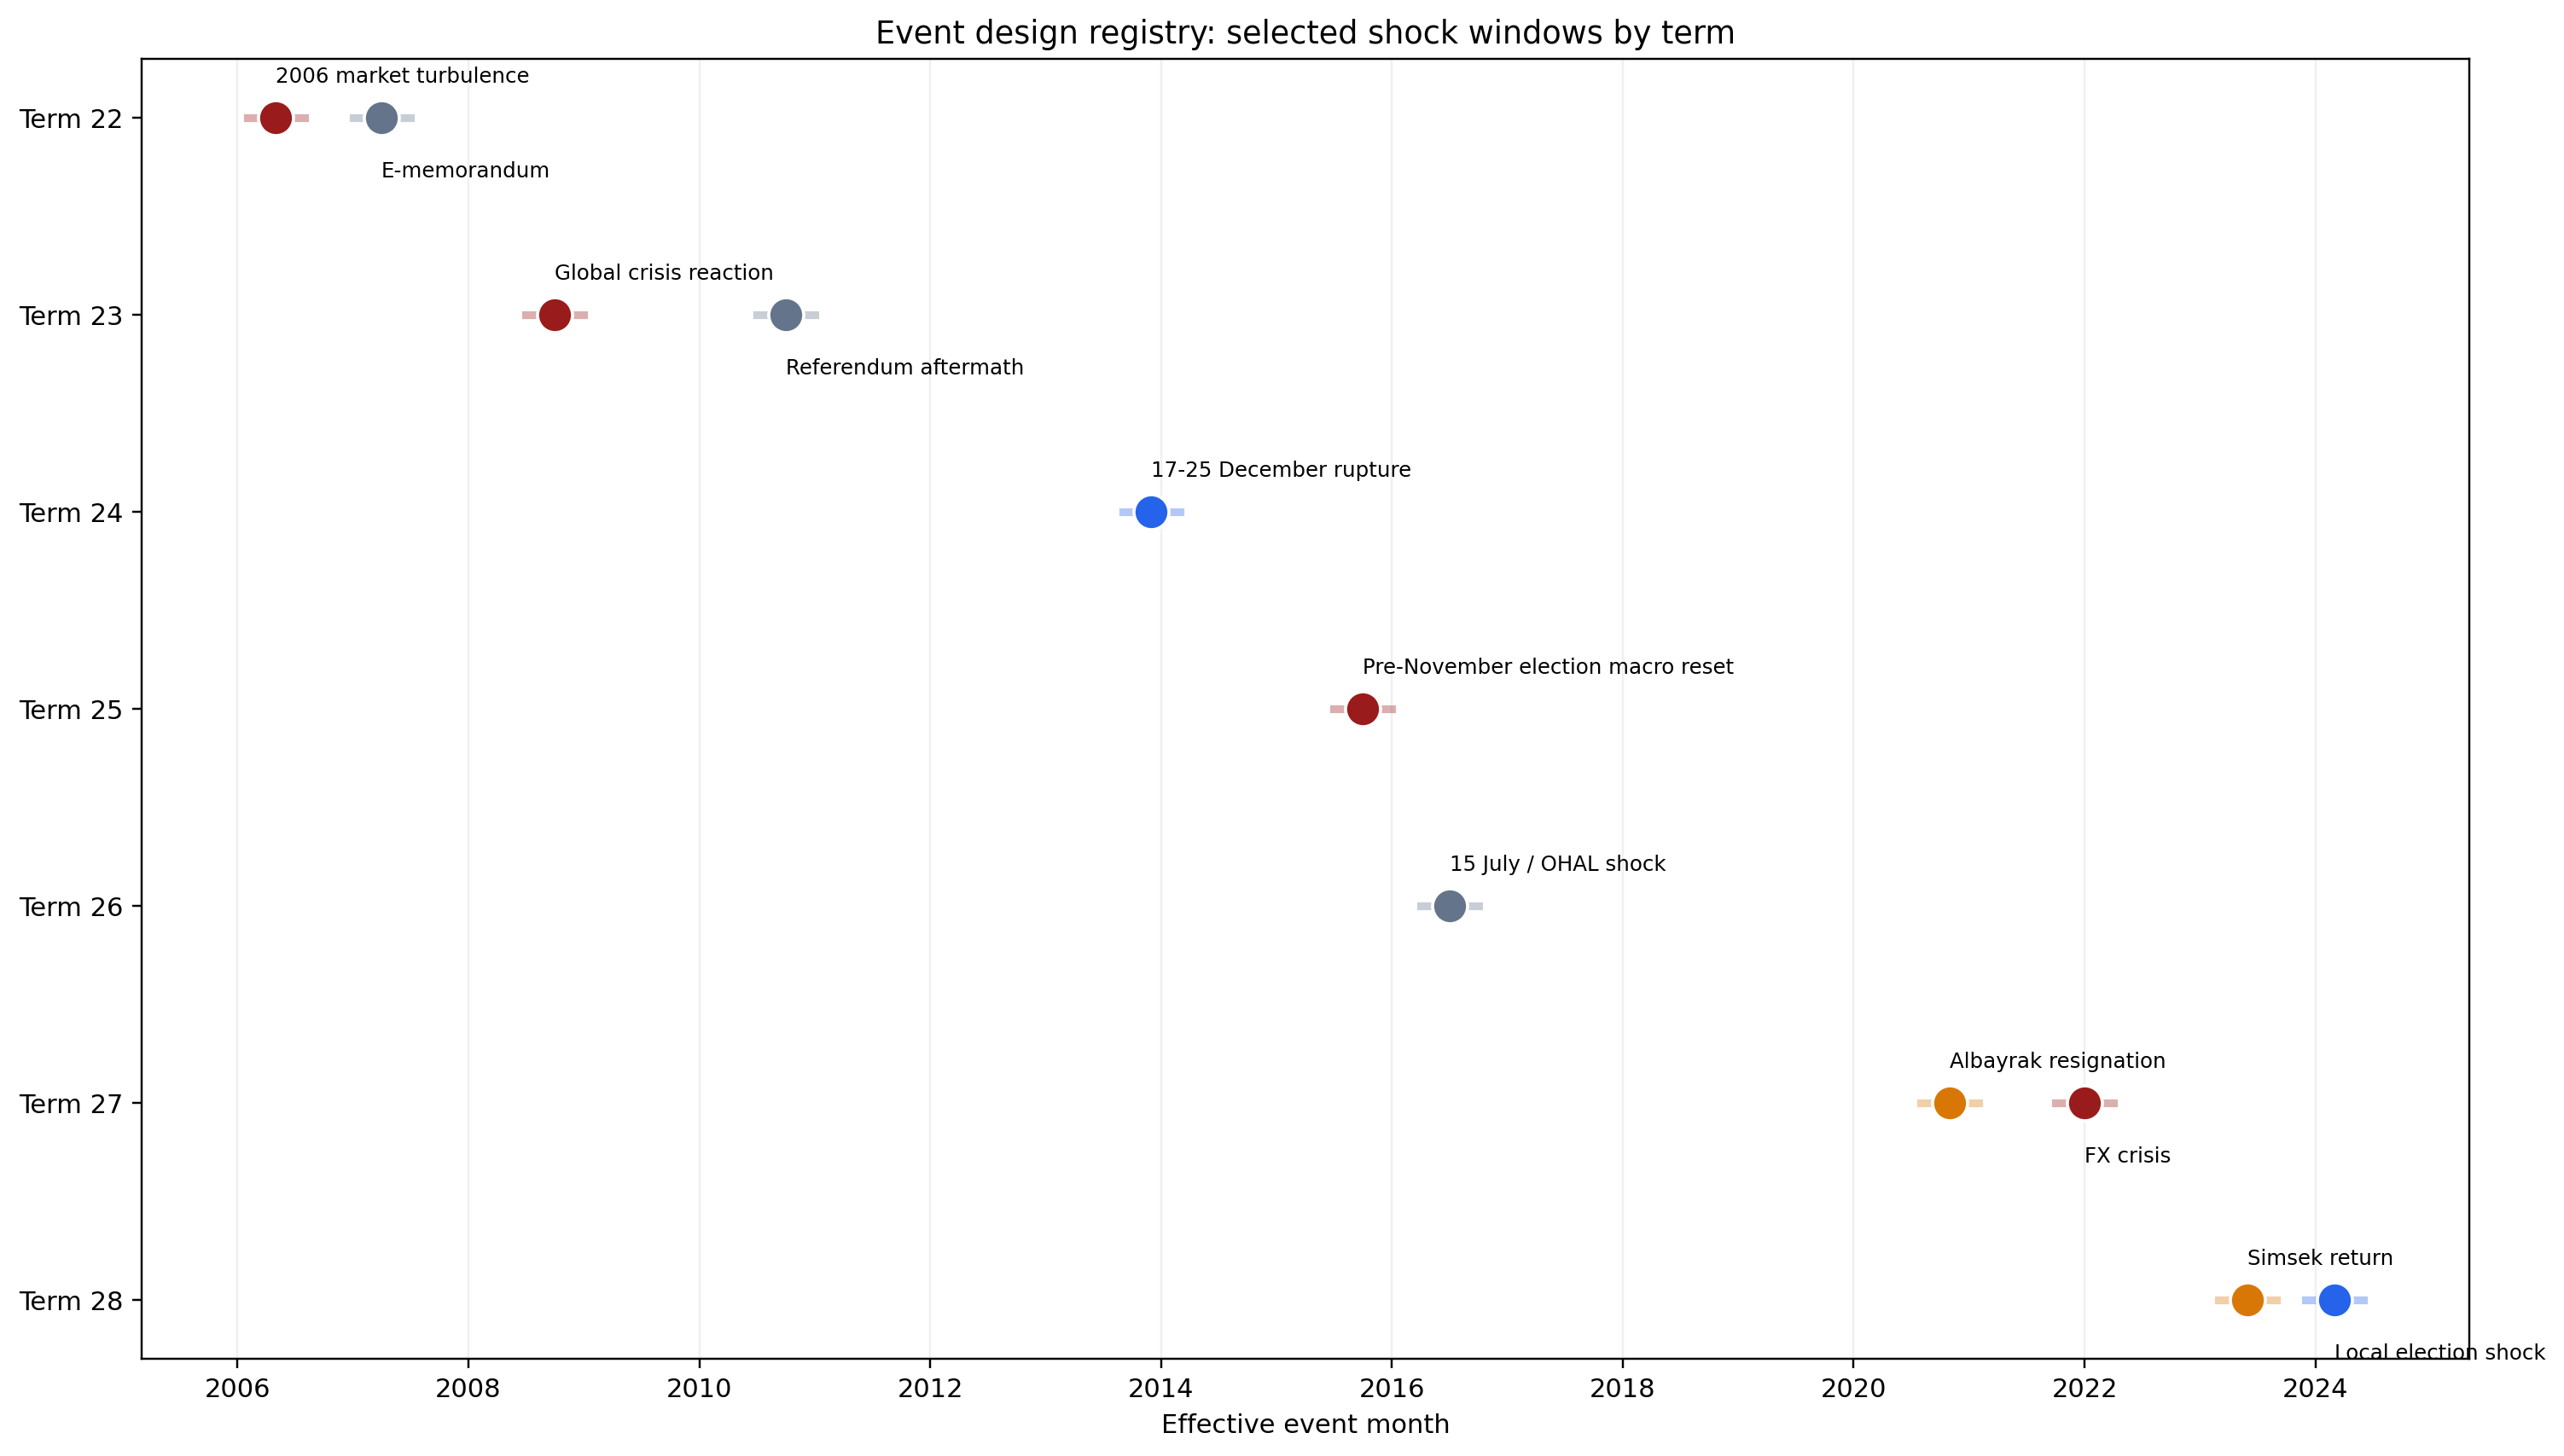
\includegraphics[width=\linewidth]{inter_term_economic_event_design.png}
    \caption{Event-centered design registry. Each marker is one shock event; the pre-shock, shock, and post-shock windows compared throughout the paper are, respectively, the 3 months before, the single month of, and the 3 months after that event -- the basic before/during/after comparison used in every later figure. Events are organized by term and shock family. Red dots mark core economic events; orange marks economic-governance events; blue marks mixed events; gray marks control events.}
    \label{fig:event_design}
\end{figure}

\section{Methods}
\subsection{Signed Agenda Feature}
The building block for everything that follows is a single number, computed for each party $p$, topic $c$, and stage $s$, that captures both how much a party talks about a topic and in what tone. We call it the signed agenda feature:
\begin{equation}
x_{p,c,s} = b_{p,c,s}\, a_{p,c,s},
\end{equation}
the product of a \emph{tone} term $b_{p,c,s}$ and a \emph{volume} term $a_{p,c,s}$. Its two ingredients are
\begin{equation}
b_{p,c,s} =
\frac{pos_{p,c,s}-neg_{p,c,s}}{pos_{p,c,s}+neg_{p,c,s}+1},
\qquad
a_{p,c,s} =
\frac{m_{p,c,s}}{\sum_{c'} m_{p,c',s}}.
\end{equation}
The tone term $b_{p,c,s}$ subtracts negative mentions from positive ones and normalizes by their total (the $+1$ avoids dividing by zero); it runs from $-1$ (all mentions negative) to $+1$ (all positive), with values near zero meaning mixed framing. The volume term $a_{p,c,s}$ is the share of party $p$'s attention spent on topic $c$ relative to all topics it raises in that stage. Multiplying the two means a party that talks a lot about a topic and frames it negatively gets a large negative $x_{p,c,s}$, while a party that barely mentions it gets a value near zero whatever its tone. Collecting these values across topics gives each party-stage a compact vector that captures volume and direction at once.

\subsection{Salience and Agenda Ownership}
Economic \emph{salience} asks how much of parliament's attention the economy commands: the share of macroeconomic topic weight among all topics in a stage,
\begin{equation}
S_{e,s} = \frac{mentions_{\text{macro},e,s}}{\sum_k mentions_{k,e,s}},
\qquad
\Delta S_e = S_{e,\text{shock}} - S_{e,\text{pre}}.
\end{equation}
$S_{e,s}$ ranges from 0 (the economy is absent from the chamber) to 1 (nothing else is discussed), and $\Delta S_e$ measures how far that share moved from the pre-shock to the shock window. A positive $\Delta S_e$ means the shock pulled attention toward economic language. This is the paper's basic test of whether a shock ``shows up'' in discourse before we ask who controls it.

Agenda \emph{ownership} asks who controls that conversation. It is the share of all economy-topic mentions in a stage that come from a single party,
\begin{equation}
O_{p,e,s} =
\frac{\sum_{c \in C_{\text{econ}}} m_{p,c,e,s}}
{\sum_{p'} \sum_{c \in C_{\text{econ}}} m_{p',c,e,s}},
\end{equation}
so the values across parties add up to one. A party with high $O_{p,e,s}$ is effectively setting the terms of the economic debate, regardless of whether its framing is positive or negative. Salience and ownership are distinct: the whole chamber can be talking about the economy (high $S_{e,s}$) while that talk is dominated by one party or spread evenly. We summarize how concentrated ownership is with a Herfindahl-Hirschman index,
\begin{equation}
HHI_{e,s} = \sum_p O_{p,e,s}^2,
\end{equation}
which is high when one or two parties dominate and low when ownership is even, plus a persistence indicator for whether the shock-window owner is still the owner afterward.

\subsection{Party-Party Affinity and Distance}
The next question is how alike two parties sound on the economy -- whether they emphasize and frame the same topics the same way, or pull in opposite directions. After standardizing the agenda-feature vectors within the pooled economic feature space, we measure affinity by cosine similarity,
\begin{equation}
A_{ij,s} =
\frac{\tilde{x}_{i,s}\cdot\tilde{x}_{j,s}}
{\|\tilde{x}_{i,s}\|_2 \|\tilde{x}_{j,s}\|_2},
\end{equation}
which compares the \emph{direction} of two parties' vectors rather than their size. $A_{ij,s}$ is near $+1$ when $i$ and $j$ stress and frame the same topics alike, near $-1$ when they stress the same topics in opposite tones, and near 0 when their agendas barely overlap. These values define the party-party network: positive affinities become cooperative edges, negative ones become conflict edges.

Two complementary summaries describe how polarized the system looks. Partisan \emph{distance} is the spread of parties on a common latent economic axis (Section~3.6), $D_s = \max_p \pi_{p,s} - \min_p \pi_{p,s}$, where $\pi_{p,s}$ is party $p$'s position; a larger $D_s$ means the field has widened. The \emph{negative-edge share} instead measures how much of the relationship structure is openly adversarial,
\begin{equation}
NES_s =
\frac{\sum_{i<j} |A_{ij,s}|\, \mathbf{1}[A_{ij,s}<0]}
{\sum_{i<j} |A_{ij,s}|}.
\end{equation}
The paper's central finding -- that shocks \emph{reconfigure} rather than uniformly widen the field -- rests on the fact that these two can move in opposite directions: a shock can compress parties toward a shared crisis vocabulary (lower $D_s$) while the share of hostile relationships among them stays high or rises (higher $NES_s$).

\subsection{Structural Brokerage}
We next ask which speakers act as \emph{bridges} between two opposing camps. The camps are not assumed in advance: for each stage we build a sparse signed speaker-affinity graph, take its leading eigenvector, and split speakers by thresholding that eigenvector, leaving a neutral remainder in the middle. For each speaker $i$, let $r_i^+$ and $r_i^-$ count cross-cutting reach into the two camps. A speaker is a good broker when those two are both large and balanced, which we capture with
\begin{equation}
\beta_i = \frac{\min(r_i^+,r_i^-)}{r_i^+ + r_i^- + \varepsilon},
\qquad
GK_i = \log\!\left(1 + 25(r_i^+ + r_i^-)\right)\beta_i\, \nu_i.
\end{equation}
The balance $\beta_i$ is near 1 when a speaker reaches both camps about equally and near 0 when ties are one-sided ($\varepsilon$ avoids dividing by zero). The gatekeeper score $GK_i$ combines that balance with overall reach on a diminishing-returns (logarithmic) scale, and $\nu_i$ gives a small boost to speakers in the neutral remainder. A high $GK_i$ thus marks a genuine bridge with substantial reach into \emph{both} sides, not merely a well-connected member of one camp. Averaging $GK_i$ over a party's speakers gives that party's brokerage role; the paper tracks turnover in who holds the highest score across shock windows.

\subsection{Displacement}
The displacement test asks whether competing constitutional or security frames crowd the economy out of the agenda. The economy's own salience change is
\begin{equation}
\Delta E_e = S^{\text{shock}}_{\text{economy},e} - S^{\text{pre}}_{\text{economy},e},
\end{equation}
positive when the economy grew during the shock and negative when economic talk actually shrank. Against this we set the combined growth of competing frames -- counting only the topics that \emph{grew} -- and subtract the economy's own gain:
\begin{equation}
G_e = \max(0,\Delta C_e) + \max(0,\Delta S_e),
\qquad
DI_e = G_e - \Delta E_e,
\end{equation}
where $\Delta C_e$ and $\Delta S_e$ are the shock-pre changes in constitutional and security topic shares. A positive displacement index $DI_e$ means competing frames grew more than the economy did, so the agenda reorganized around something other than the economic story even when the shock itself was economic; a negative $DI_e$ means the economy stayed the dominant organizing topic. This is the formal version of the paper's claim that objective economic pressure does not automatically translate into economic centrality.

\subsection{Inter-Term Latent Axis and Robustness}
To compare party positions across terms, all party-year-topic observations from Terms 22--28 are pooled and standardized. An anchor-guided weight vector is estimated from correlations between anchor-party mean profiles and anchor-direction scores, producing a common economy-specific latent axis for inter-term position and drift. Robustness is assessed with within-term placebo months, bootstrap stability checks, anchor permutation, and leave-one-anchor-out diagnostics.

\subsection{Hypotheses}
The five hypotheses are not an arbitrary checklist: each operationalizes one of the three mechanisms named in the Introduction, grounded in a tradition from Related Work. H1 and H2 target agenda ownership -- whether a shock pulls economic language toward the center of debate, and who ends up controlling it -- following agenda-setting theory's separation of salience from control \cite{kleinnijenhuis1995}. H3 targets partisan distance, drawing on signed and polarized network analysis \cite{bonchi2019, blohm2026}. H4 targets structural brokerage, extending network analyses of legislative bodies \cite{porter2005} to dynamic bridging under stress. H5 is a complementary boundary-condition hypothesis: the mixed and control events exist precisely so the analysis can ask whether economic pressure wins the agenda, or can be displaced by non-economic frames. Crucially, every hypothesis is written as non-directional and falsifiable either way -- H3 predicts \emph{reconfiguration}, not widening -- so the data can reveal heterogeneous effects rather than a single forced direction. Table~\ref{tab:hypotheses} summarizes each hypothesis and where it is tested.

\begin{table}[htbp]
\centering
\caption{Hypotheses and where each is tested.}
\label{tab:hypotheses}
\small
\begin{tabular}{p{0.05\linewidth} p{0.64\linewidth} p{0.22\linewidth}}
\toprule
\textbf{H} & \textbf{Claim} & \textbf{Tested in} \\
\midrule
H1 & External shocks raise the salience of macroeconomic discourse in parliament. & Results 5.1, salience shift \\
H2 & External shocks redistribute agenda ownership between government and opposition, not necessarily toward government. & Results 5.1, ownership reallocation \\
H3 & External shocks reconfigure partisan distance in discourse space, widening or compressing it. & Results 5.2, spread and modularity \\
H4 & External shocks reassign structural brokerage; the pre-shock top broker is typically not the shock-window top broker. & Results 5.3, broker turnover \\
H5 & Economic pressure does not always elevate economic discourse; competing constitutional or security frames can displace it. & Results 5.4, displacement index \\
\bottomrule
\end{tabular}
\end{table}

\section{Results}
\subsection{Economic Shocks Raise Salience and Reallocate Ownership}
The clearest evidence for H1 comes from the two strongest core economic shocks. In Term 23, the global crisis reaction raises economic salience from 0.297 to 0.473, a shock-pre increase of 0.176. In Term 27, the FX crisis raises salience from 0.478 to 0.656, an equally large increase of 0.178. In both cases, macroeconomic language moves toward the center of parliamentary communication.

Agenda ownership shifts at the same time, but not according to a single government-opposition rule. In Term 23, ownership moves from CHP to AKP and stays with AKP in the post-shock window. In Term 27, it moves from CHP to IYI Party during the shock and then returns to CHP afterward. Economic salience therefore does not mechanically imply stable governmental control of the economic agenda -- it can instead trigger temporary or intra-opposition ownership reallocation. This pattern is direct evidence for H2: agenda ownership is redistributed by both shocks, but the CHP-to-AKP move in Term 23 and the CHP-to-IYI Party-to-CHP cycle in Term 27 point in different directions, confirming that shock-driven reallocation does not follow a single government-opposition trajectory.

\begin{figure}[htbp]
    \centering
    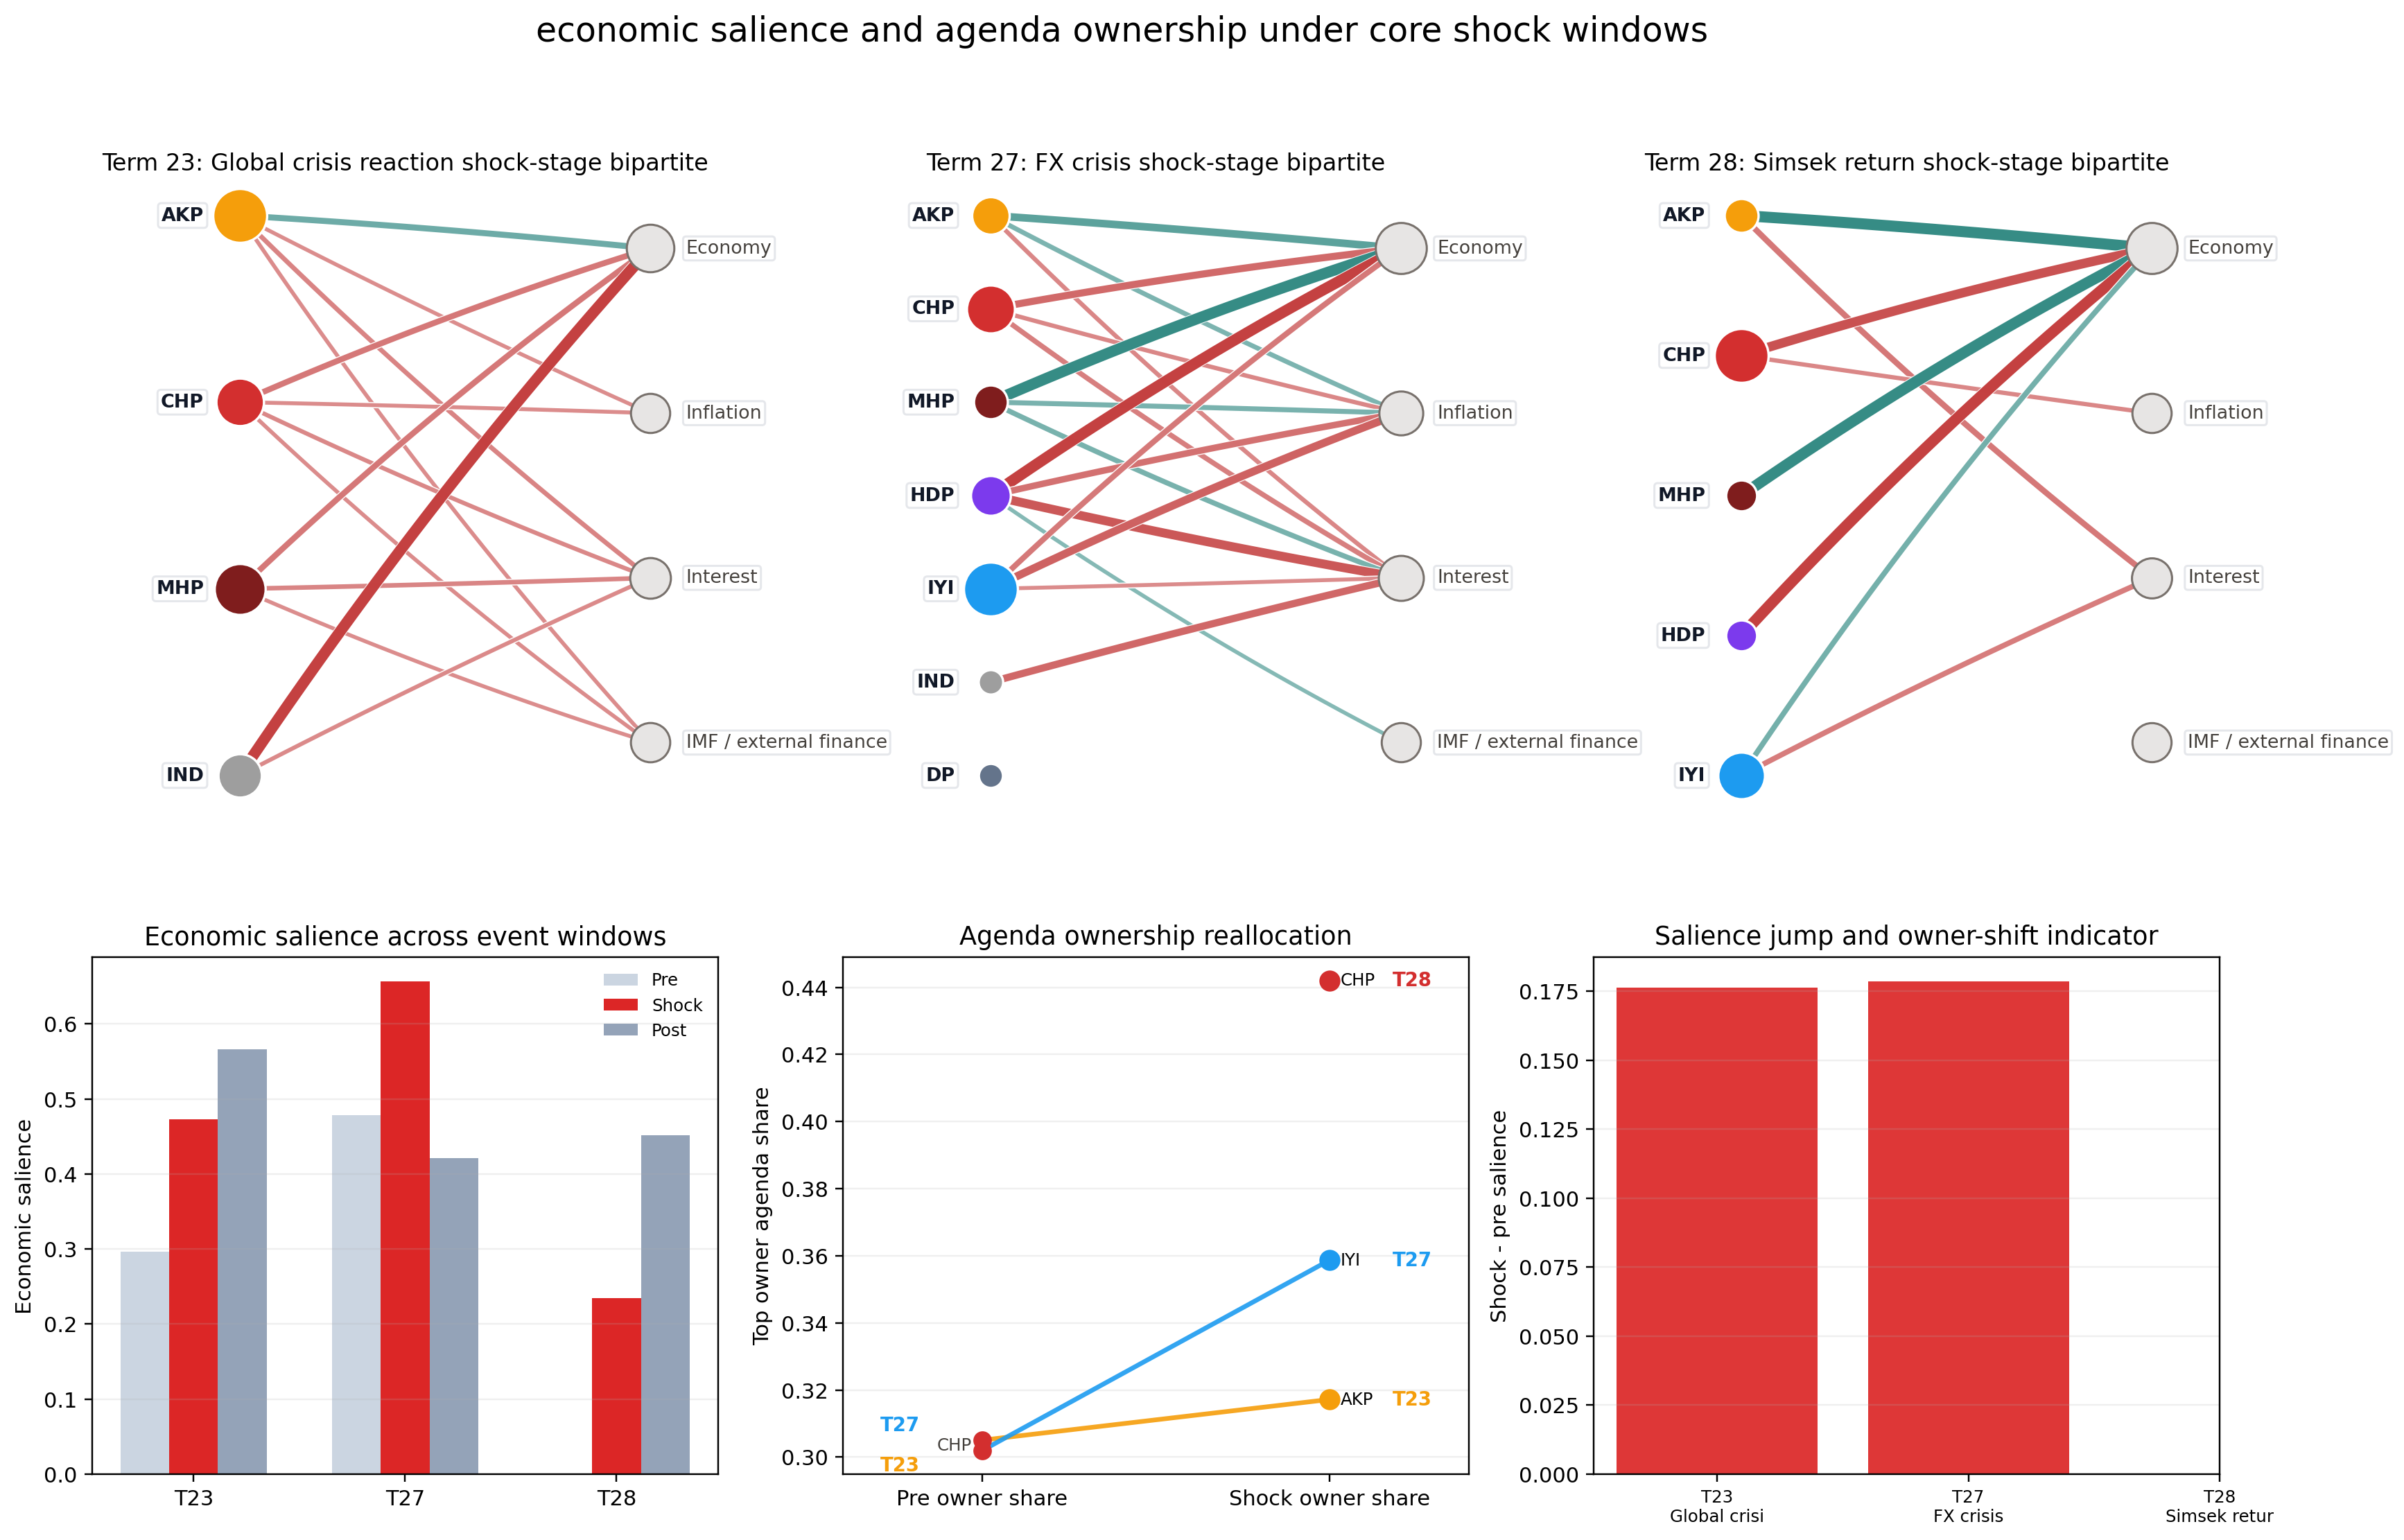
\includegraphics[width=\linewidth]{figure_6_agenda_ownership_panel.png}
    \caption{Economic salience and agenda ownership across core shock windows. \emph{Salience} is the share of parliamentary debate devoted to economic topics in a window; \emph{agenda ownership} is which party's economic agenda-share is largest. The upper row shows party-topic bipartite graphs for Terms 23, 27, and 28. The lower row compares salience levels, ownership reallocation paths, and salience jump sizes across events. In the reallocation panel (lower middle), each line runs from a party's pre-shock to shock-window agenda-share, colored by the shock-window owner.}
    \label{fig:ownership}
\end{figure}

\subsection{Partisan Distance Is Reconfigured, Not Monotonically Widened}
H3 is supported in a stronger form than a simple widening hypothesis. In Term 23, the global crisis reaction widens discourse spread from 0.862 to 1.507, and negative-edge share rises from 0.695 to 0.849. Term 28's local-election shock also widens spread, from 3.067 to 3.526.

The FX crisis in Term 27 tells a different story. Economic salience rises sharply, but spread contracts from 5.402 to 4.906 and signed modularity (how cleanly the affinity network splits into separate, internally aligned blocs) drops relative to pre-shock. This does not contradict H3 -- it shows that shocks can compress multiple parties into a denser crisis language even while keeping conflict visible. The paper's claim is reconfiguration, not one-directional widening.

Figures~\ref{fig:triptych23}--\ref{fig:triptych28} each present a \emph{triptych}: a three-panel figure showing the same party network side by side for the pre-shock, shock, and post-shock windows of a focal event. In each panel, edges are colored by the sign of the underlying party-party affinity -- blue for non-negative (aligned) ties and red for negative (conflictual) ties -- with thickness scaling with magnitude. Together, the three figures tell one story: economic shocks visibly reorganize the geometry of partisan economic discourse, but whether the network spreads apart or compresses differs by shock.

\begin{figure}[htbp]
    \centering
    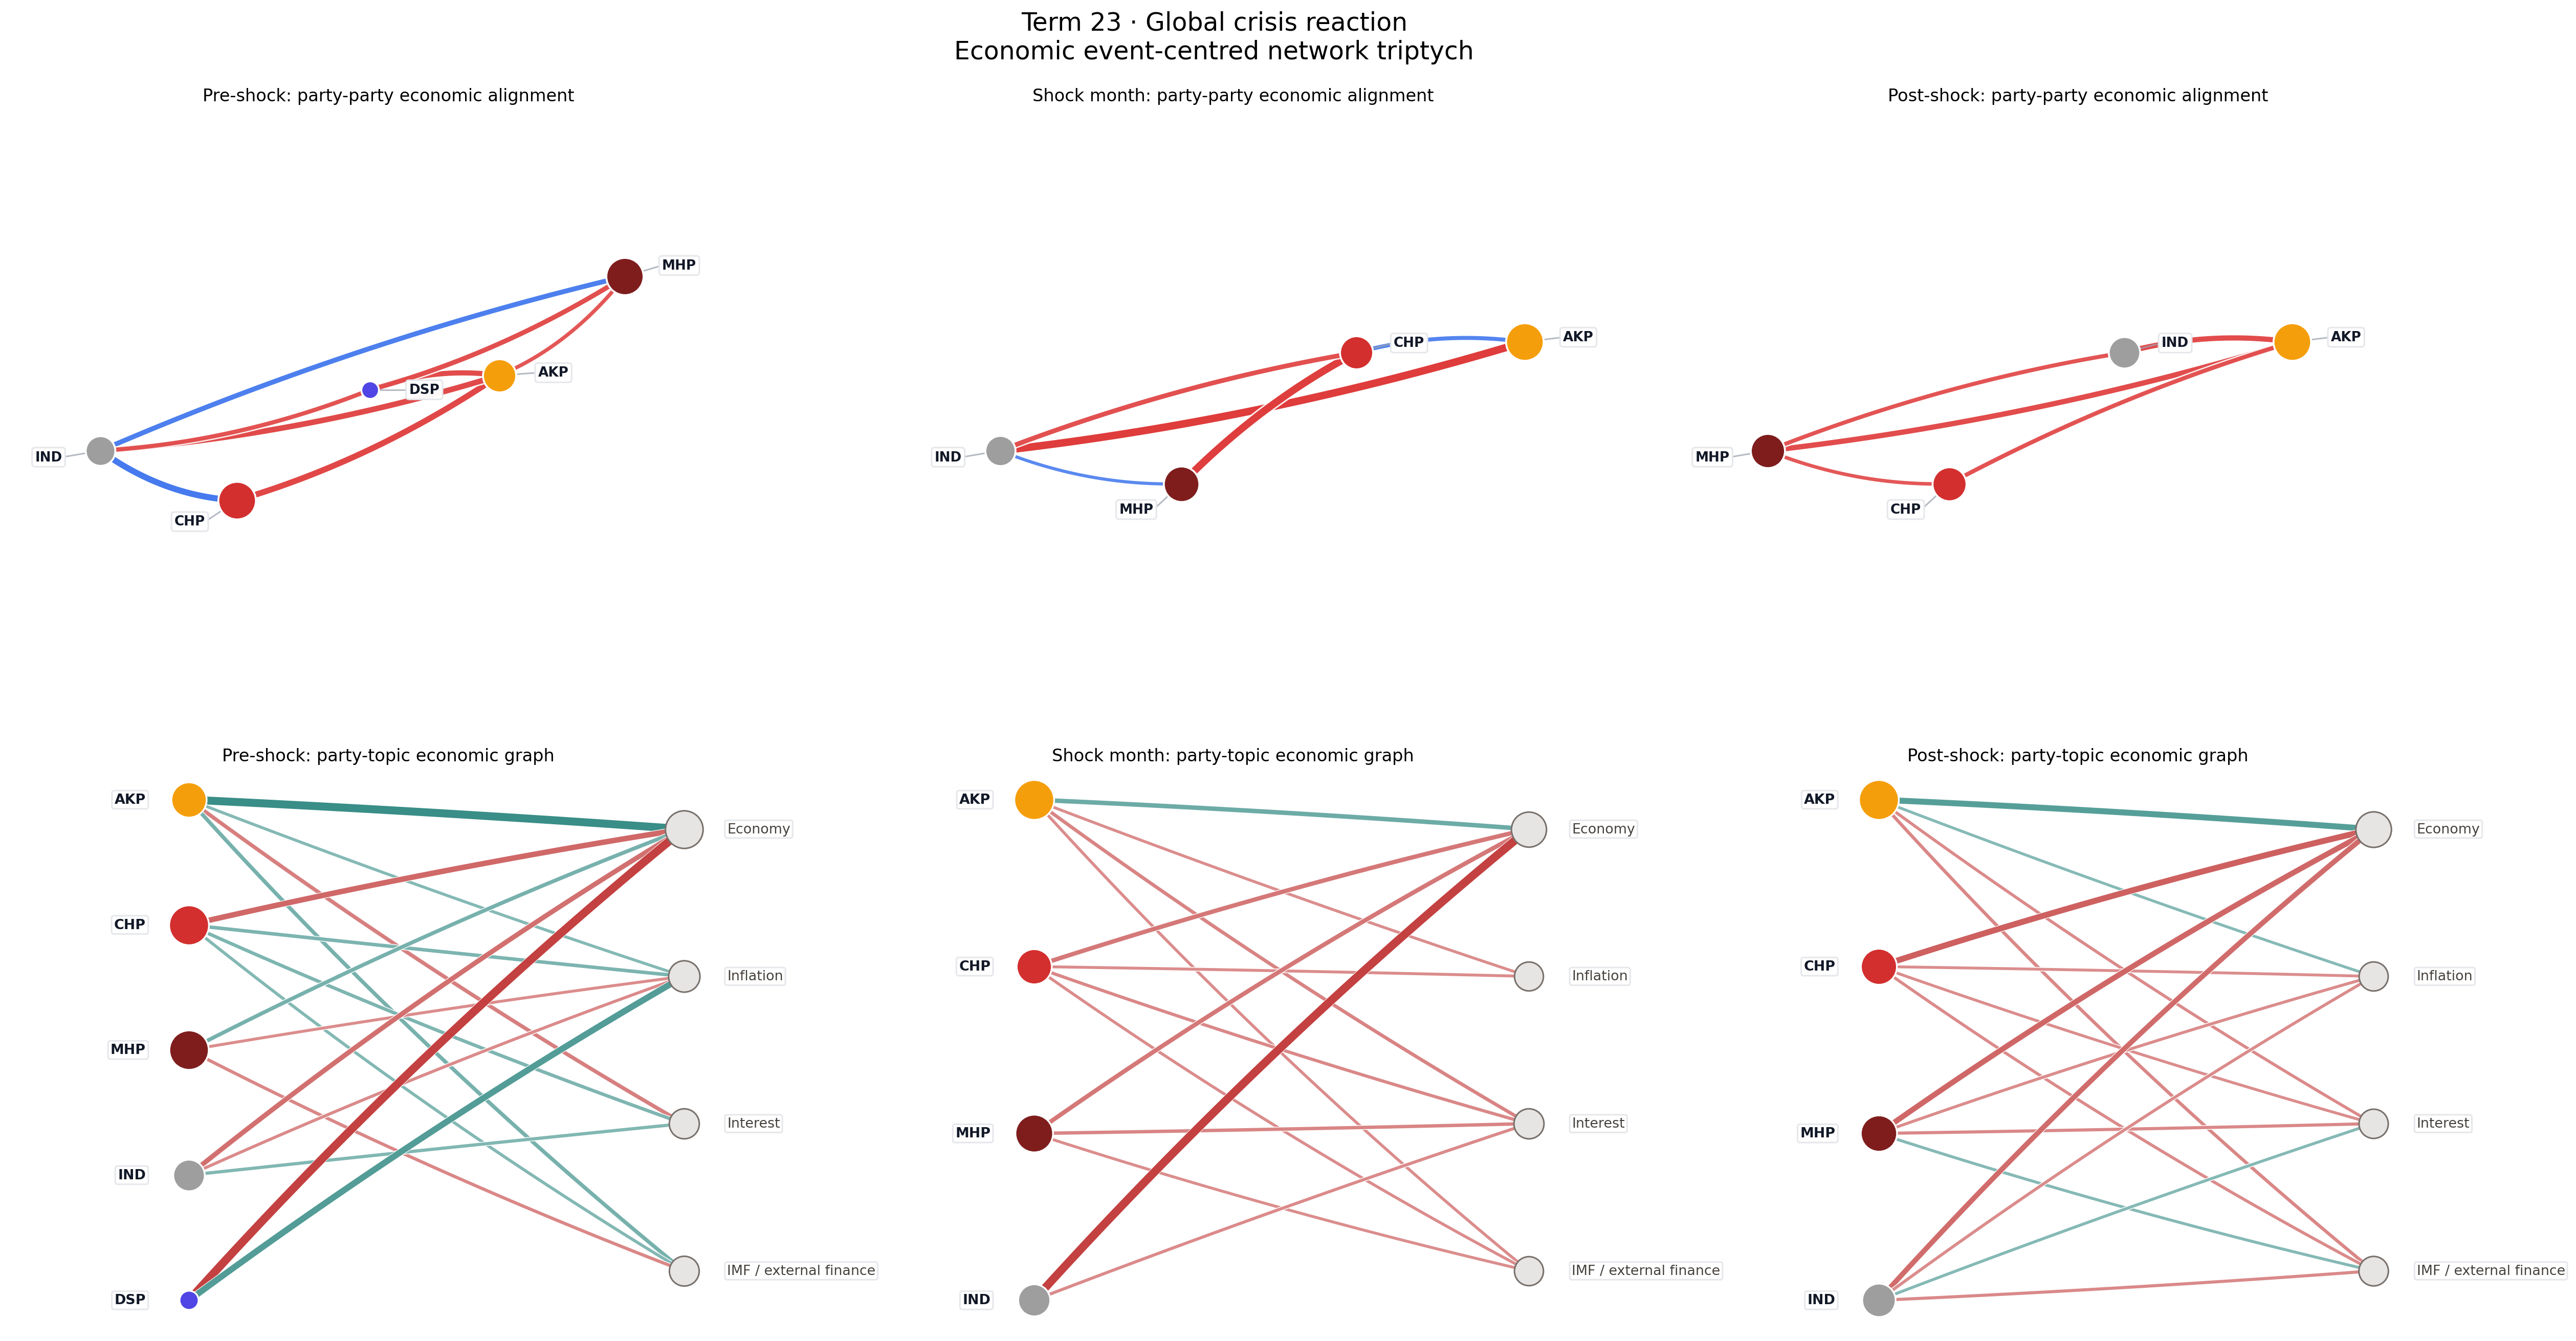
\includegraphics[width=\linewidth]{figure_3_term_23_shock_triptych.png}
    \caption{Term 23 network triptych (global crisis reaction): pre-shock, shock, and post-shock party networks side by side. Upper row: party-party economic alignment; lower row: party-topic economic structure. Edges are colored by the sign of party-party affinity -- blue for non-negative (aligned) and red for negative (conflictual) -- with thickness scaling with magnitude. Moving from pre-shock to shock, spread widens and negative-edge share rises sharply.}
    \label{fig:triptych23}
\end{figure}

\begin{figure}[htbp]
    \centering
    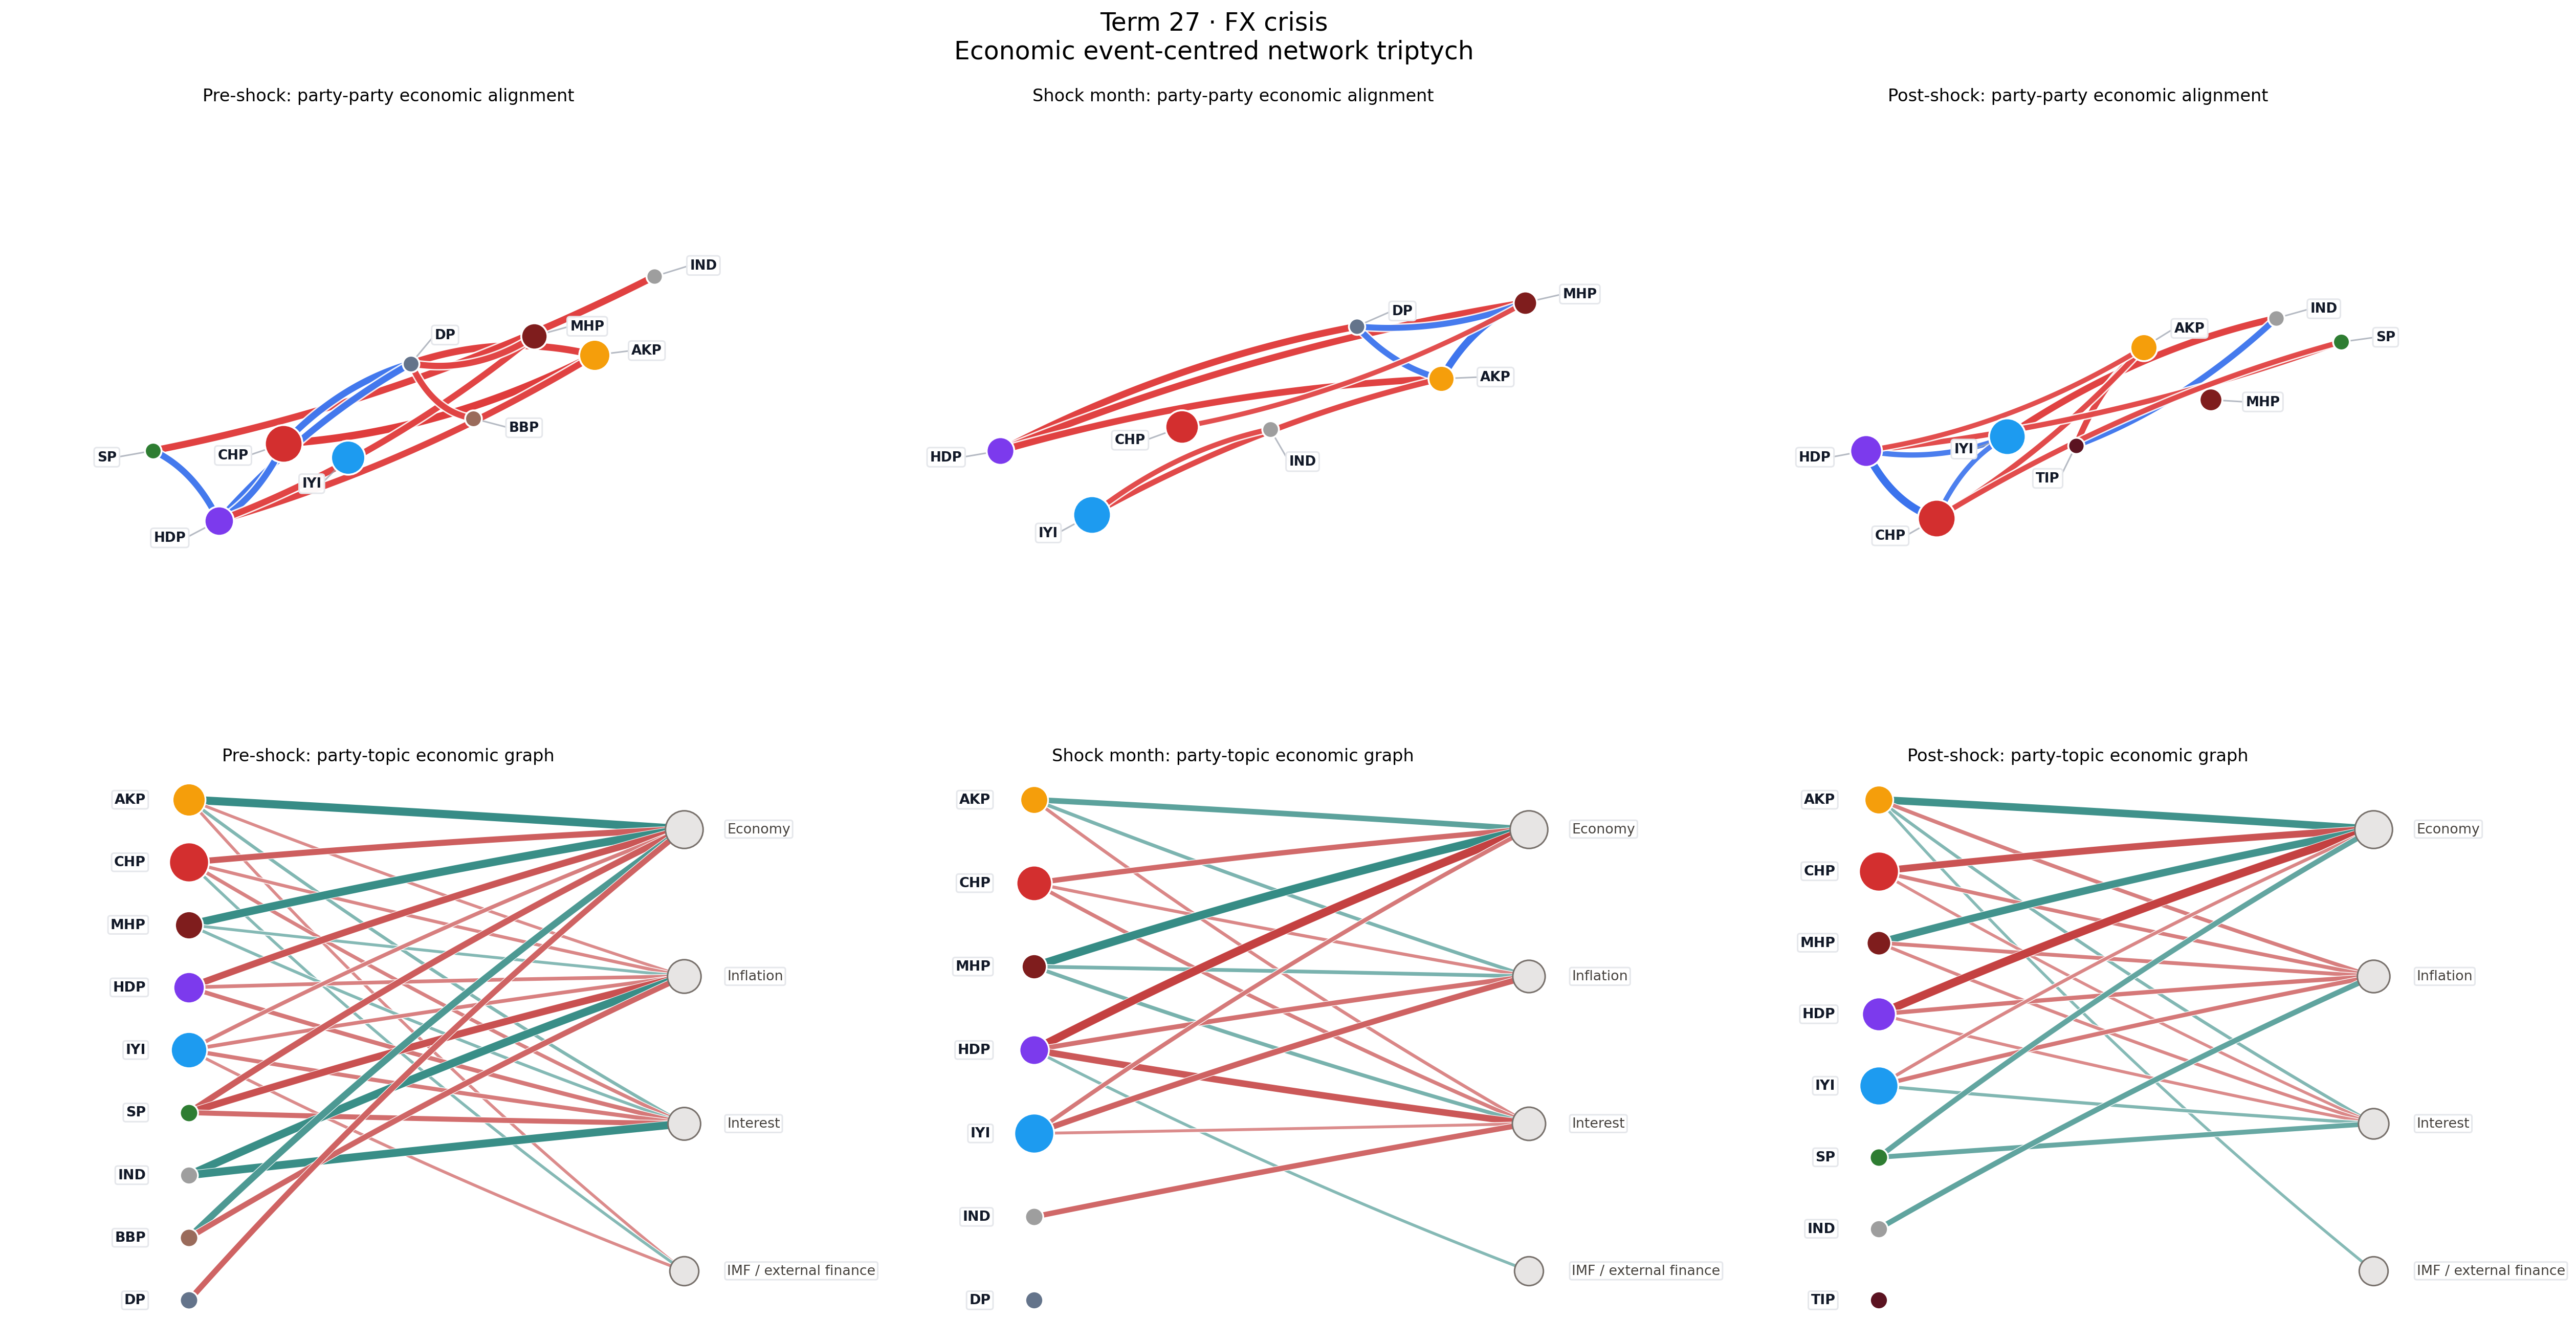
\includegraphics[width=\linewidth]{figure_4_term_27_shock_triptych.png}
    \caption{Term 27 network triptych (FX crisis): pre-shock, shock, and post-shock party networks side by side, with edges colored by the sign of party-party affinity -- blue for non-negative (aligned) and red for negative (conflictual) -- and thickness scaling with magnitude. The FX crisis produces a sharp salience rise but a more compressed discourse geometry: spread contracts rather than widens as parties converge on crisis language.}
    \label{fig:triptych27}
\end{figure}

\begin{figure}[htbp]
    \centering
    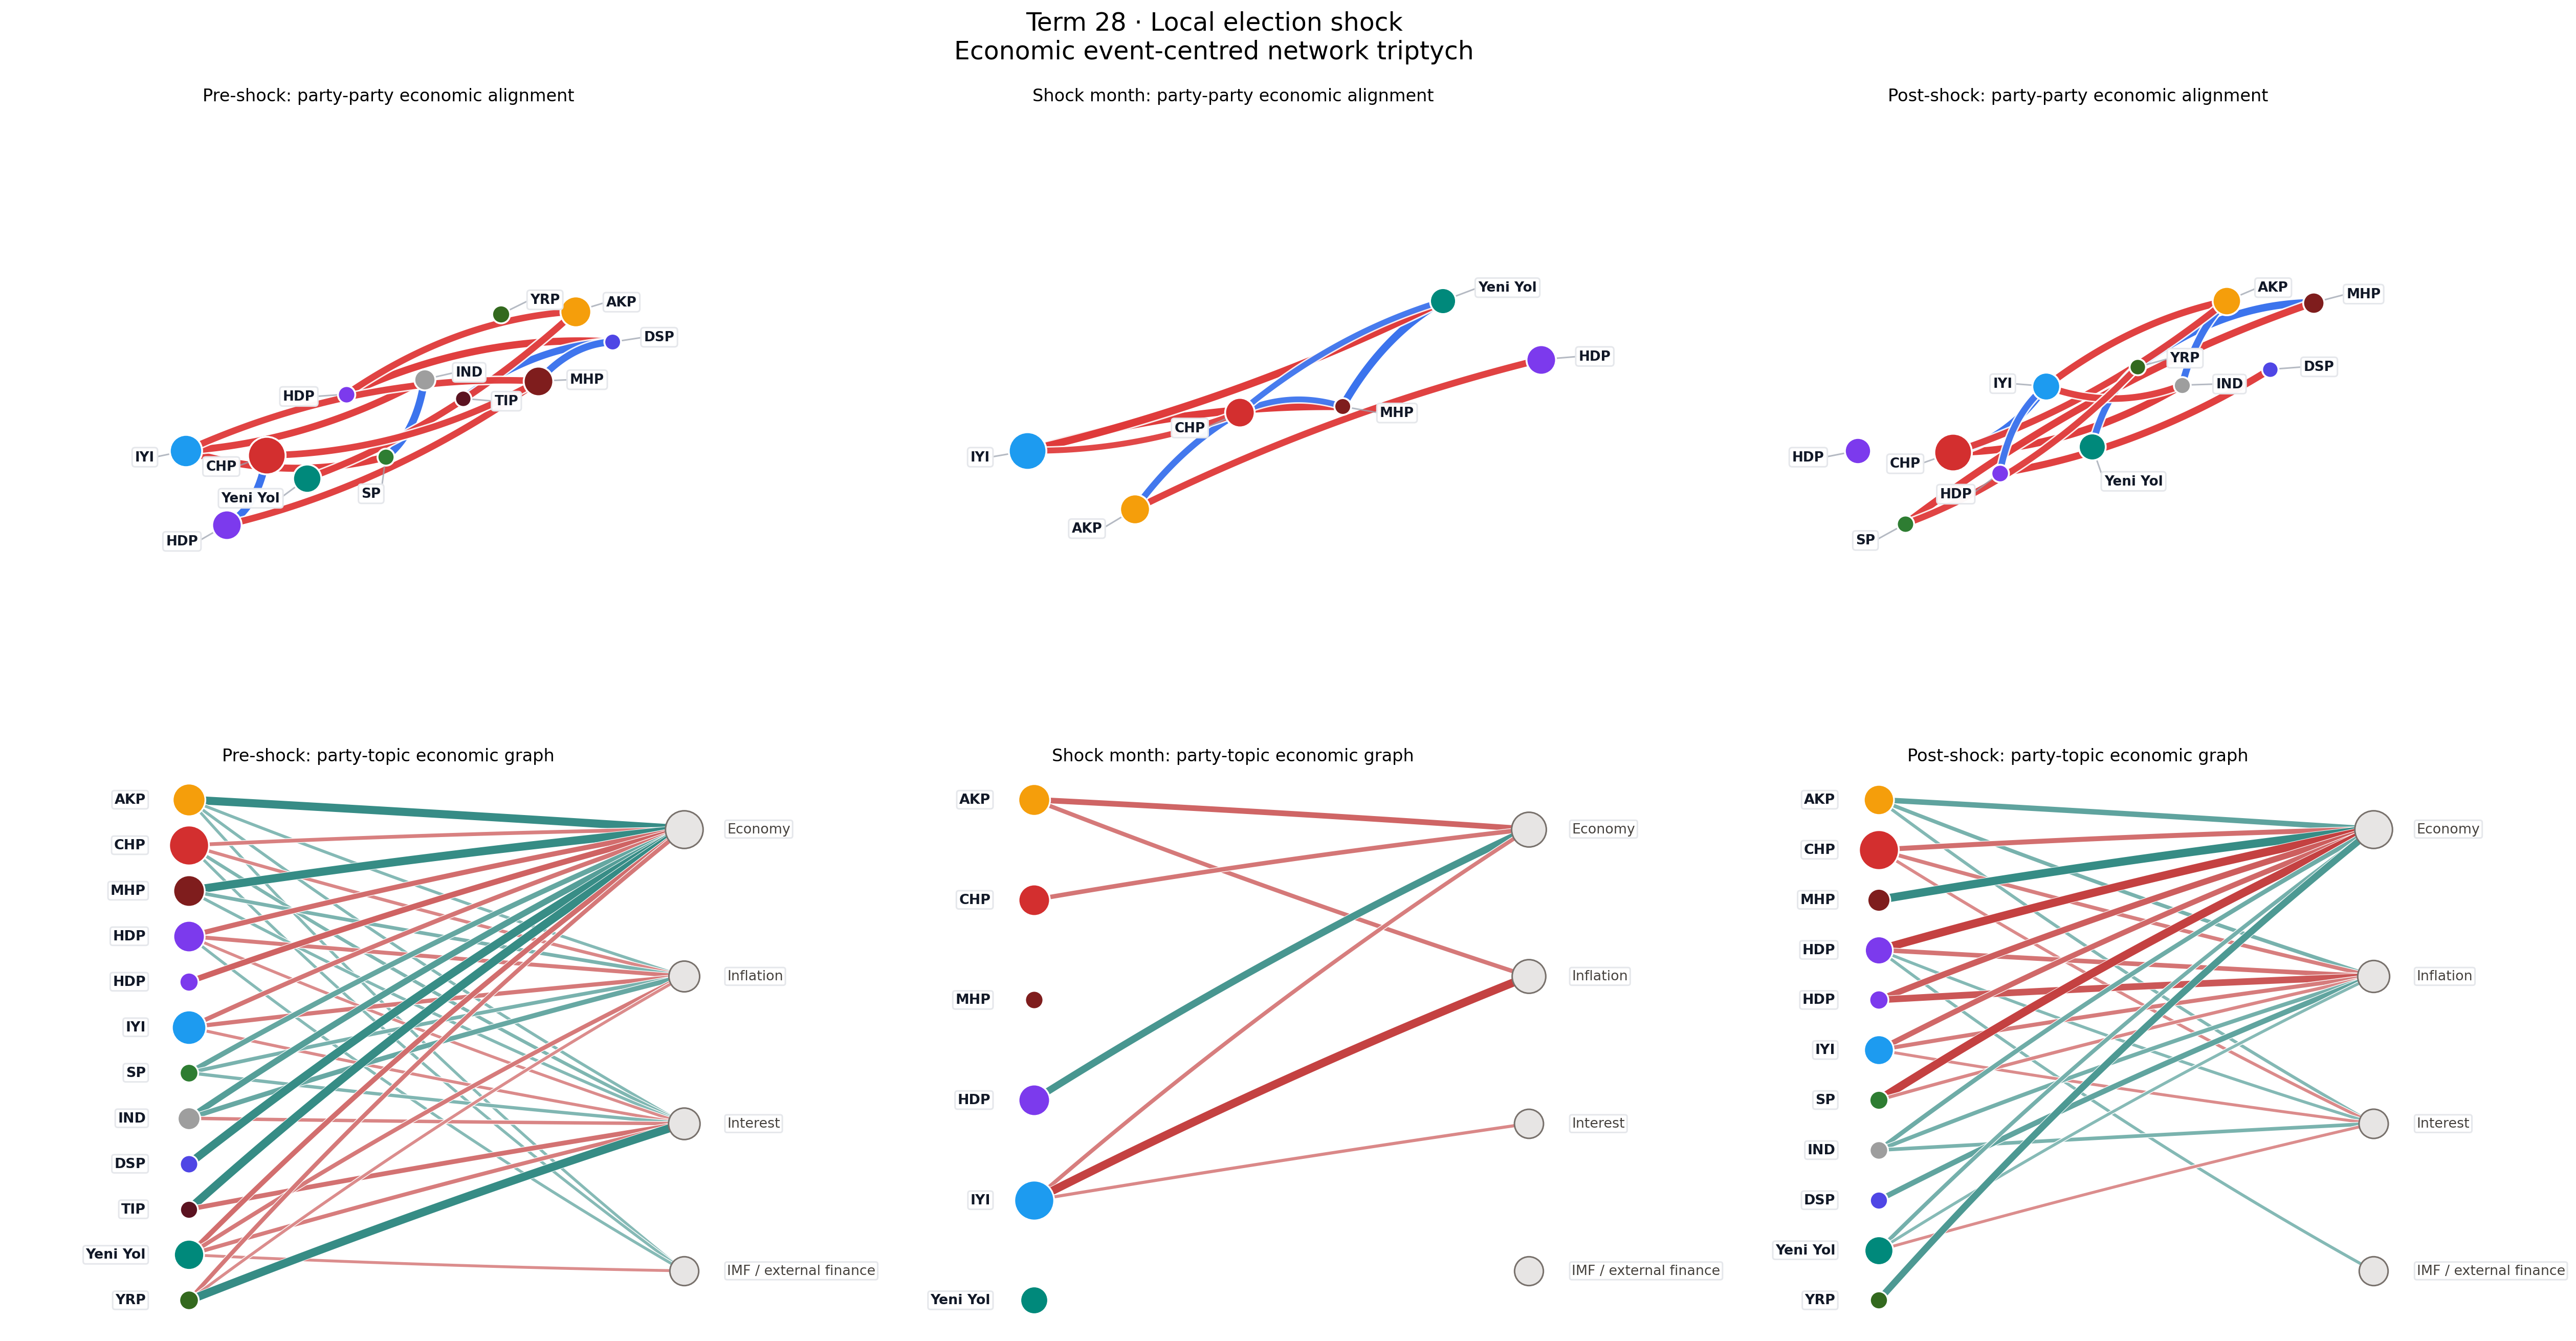
\includegraphics[width=\linewidth]{figure_5_term_28_shock_triptych.png}
    \caption{Term 28 network triptych (local-election shock): pre-shock, shock, and post-shock party networks side by side, again with edges colored by the sign of party-party affinity -- blue for non-negative (aligned) and red for negative (conflictual) -- and thickness scaling with magnitude. Spread widens moderately, and brokerage reassigns from DSP to HDP.}
    \label{fig:triptych28}
\end{figure}

\subsection{Brokerage Turns Over Under Economic Stress}
Brokerage is highly unstable across all focal shocks. In Term 23, the leading party-level broker shifts from independents to MHP. In Term 27, it shifts from DP to IYI Party. In Term 28's local-election shock, it shifts from DSP to HDP. Speaker-level broker turnover also occurs in all three cases.

These shifts matter because they show that bridging capacity is not a fixed attribute of the same centrist actor -- it is reassigned as the structure of conflict changes. Top-broker persistence is false in all three focal cases, indicating that shock-period brokerage is typically temporary rather than durable. This is the core evidence for H4: the leading party-level broker changes identity in every focal shock, and persistence is false throughout, so the pre-shock top broker is never the shock-window top broker.

\begin{figure}[htbp]
    \centering
    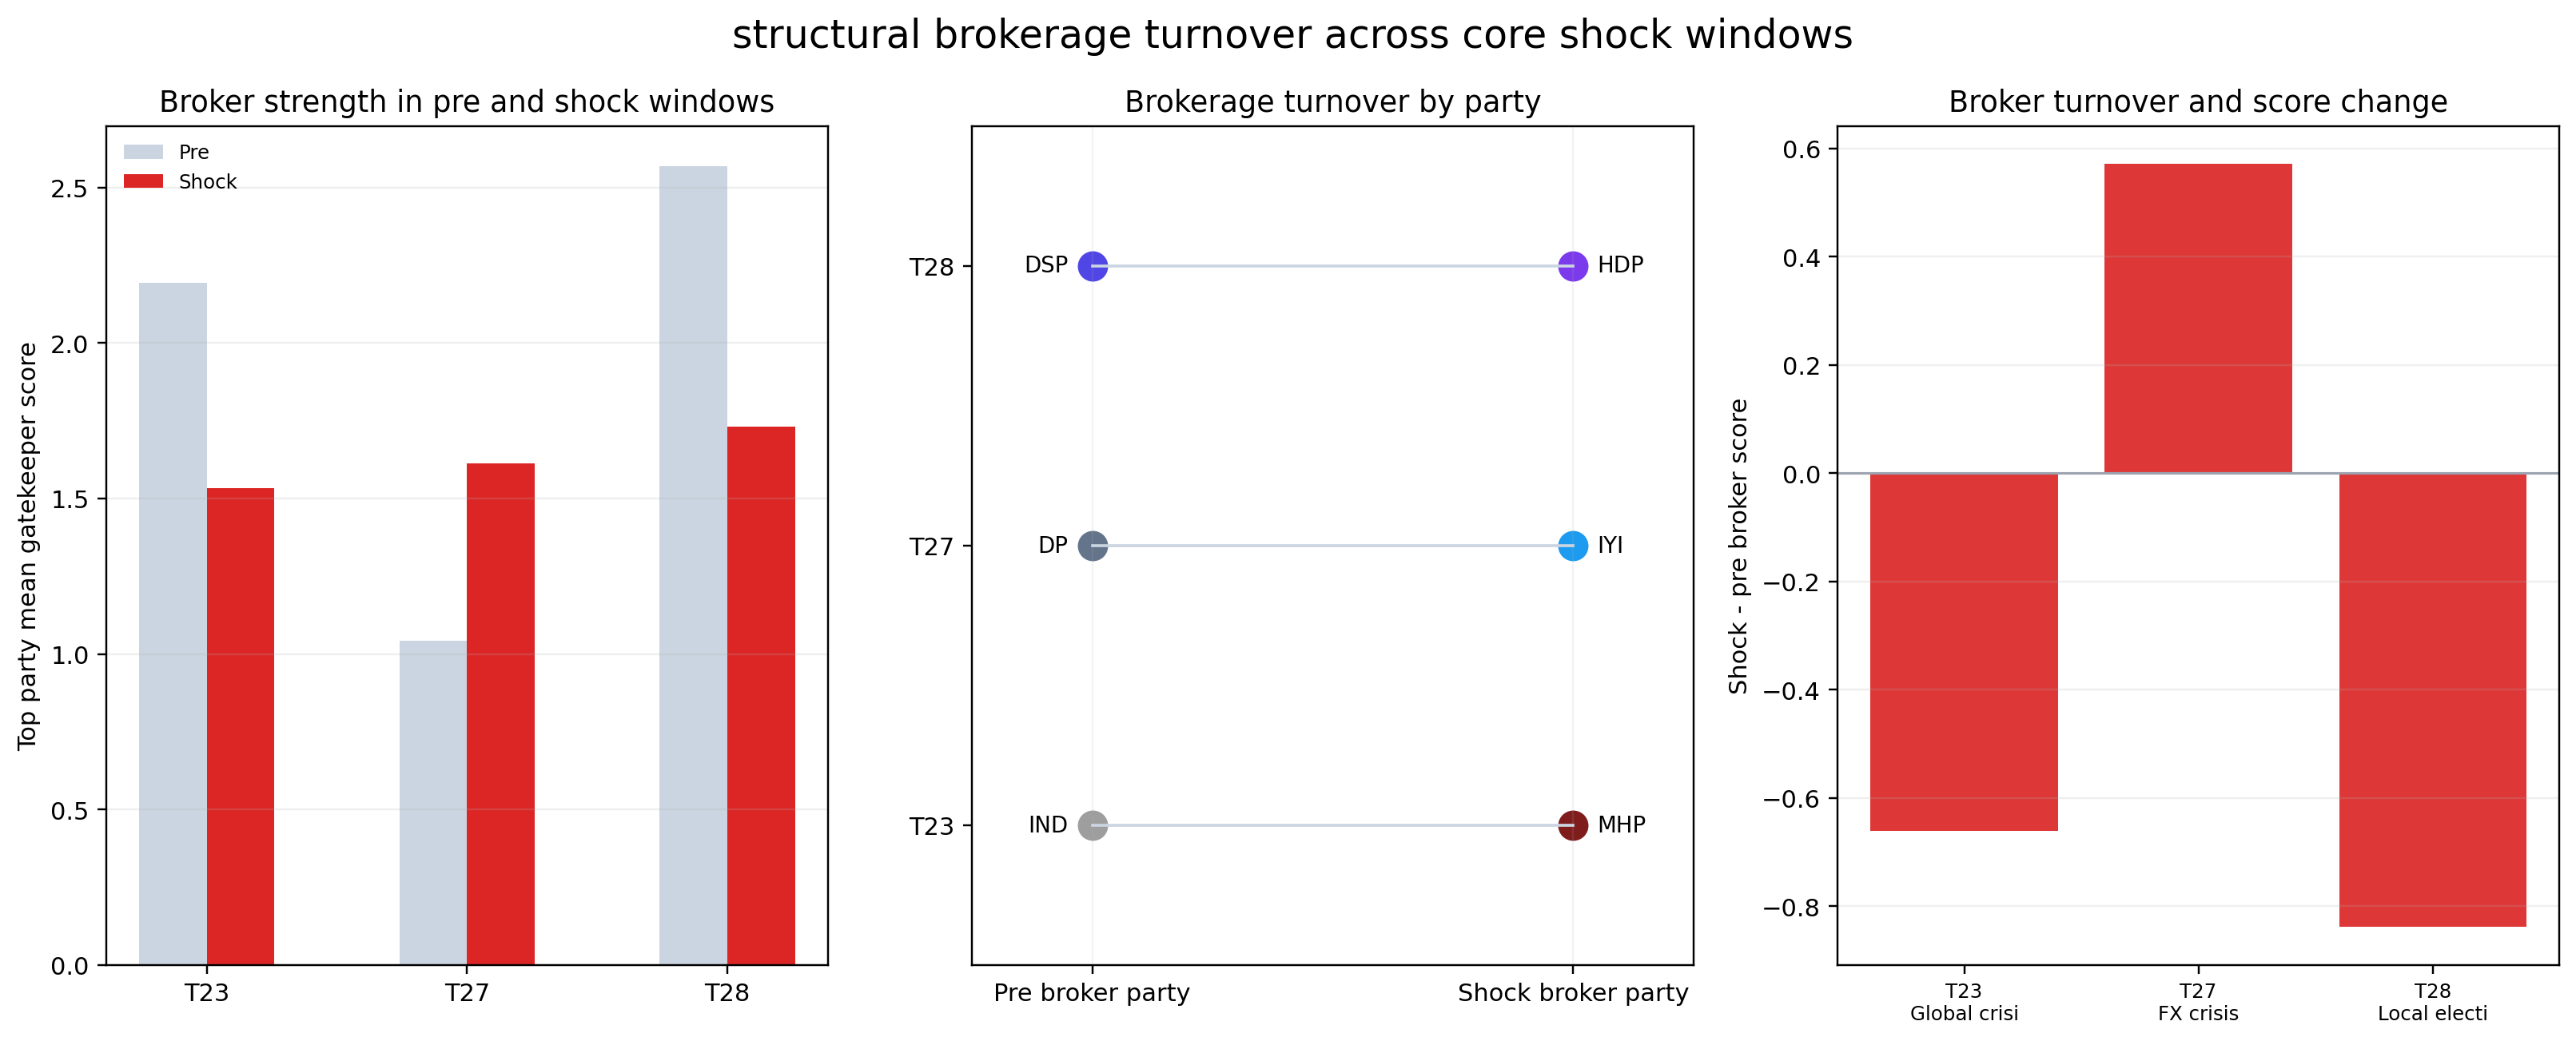
\includegraphics[width=\linewidth]{figure_7_brokerage_turnover_panel.png}
    \caption{Structural brokerage turnover across core shock windows. A party's gatekeeper score ($GK_i$, averaged across speakers; see Methods) reflects how evenly its speakers' ties split across the two opposing camps: a high score means speakers bridge both sides rather than aligning mostly with one. Left: broker strength in pre and shock windows. Center: party-level broker turnover from pre to shock. Right: net change in broker score by event.}
    \label{fig:brokerage}
\end{figure}

\subsection{Economic Pressure Does Not Always Produce Economic Centrality}
H5 is clearest in the mixed and control events. The 2007 e-memorandum is the strongest displacement case. Economic salience falls by 0.125, while constitutional and security themes jointly rise enough to produce a positive displacement index of 0.190 in the shock window. This is genuine displacement rather than a simple decline in economic talk, because competing crisis frames become more central at the same time.

Core economic shocks look different. The global crisis reaction and the FX crisis both keep negative displacement scores in the shock window, meaning the economy remains the dominant organizing layer even when other topics also rise. The contrast between event families is the key finding: objective macro pressure is not sufficient on its own -- the parliamentary field can still be reorganized around constitutional or security conflict.

\begin{figure}[htbp]
    \centering
    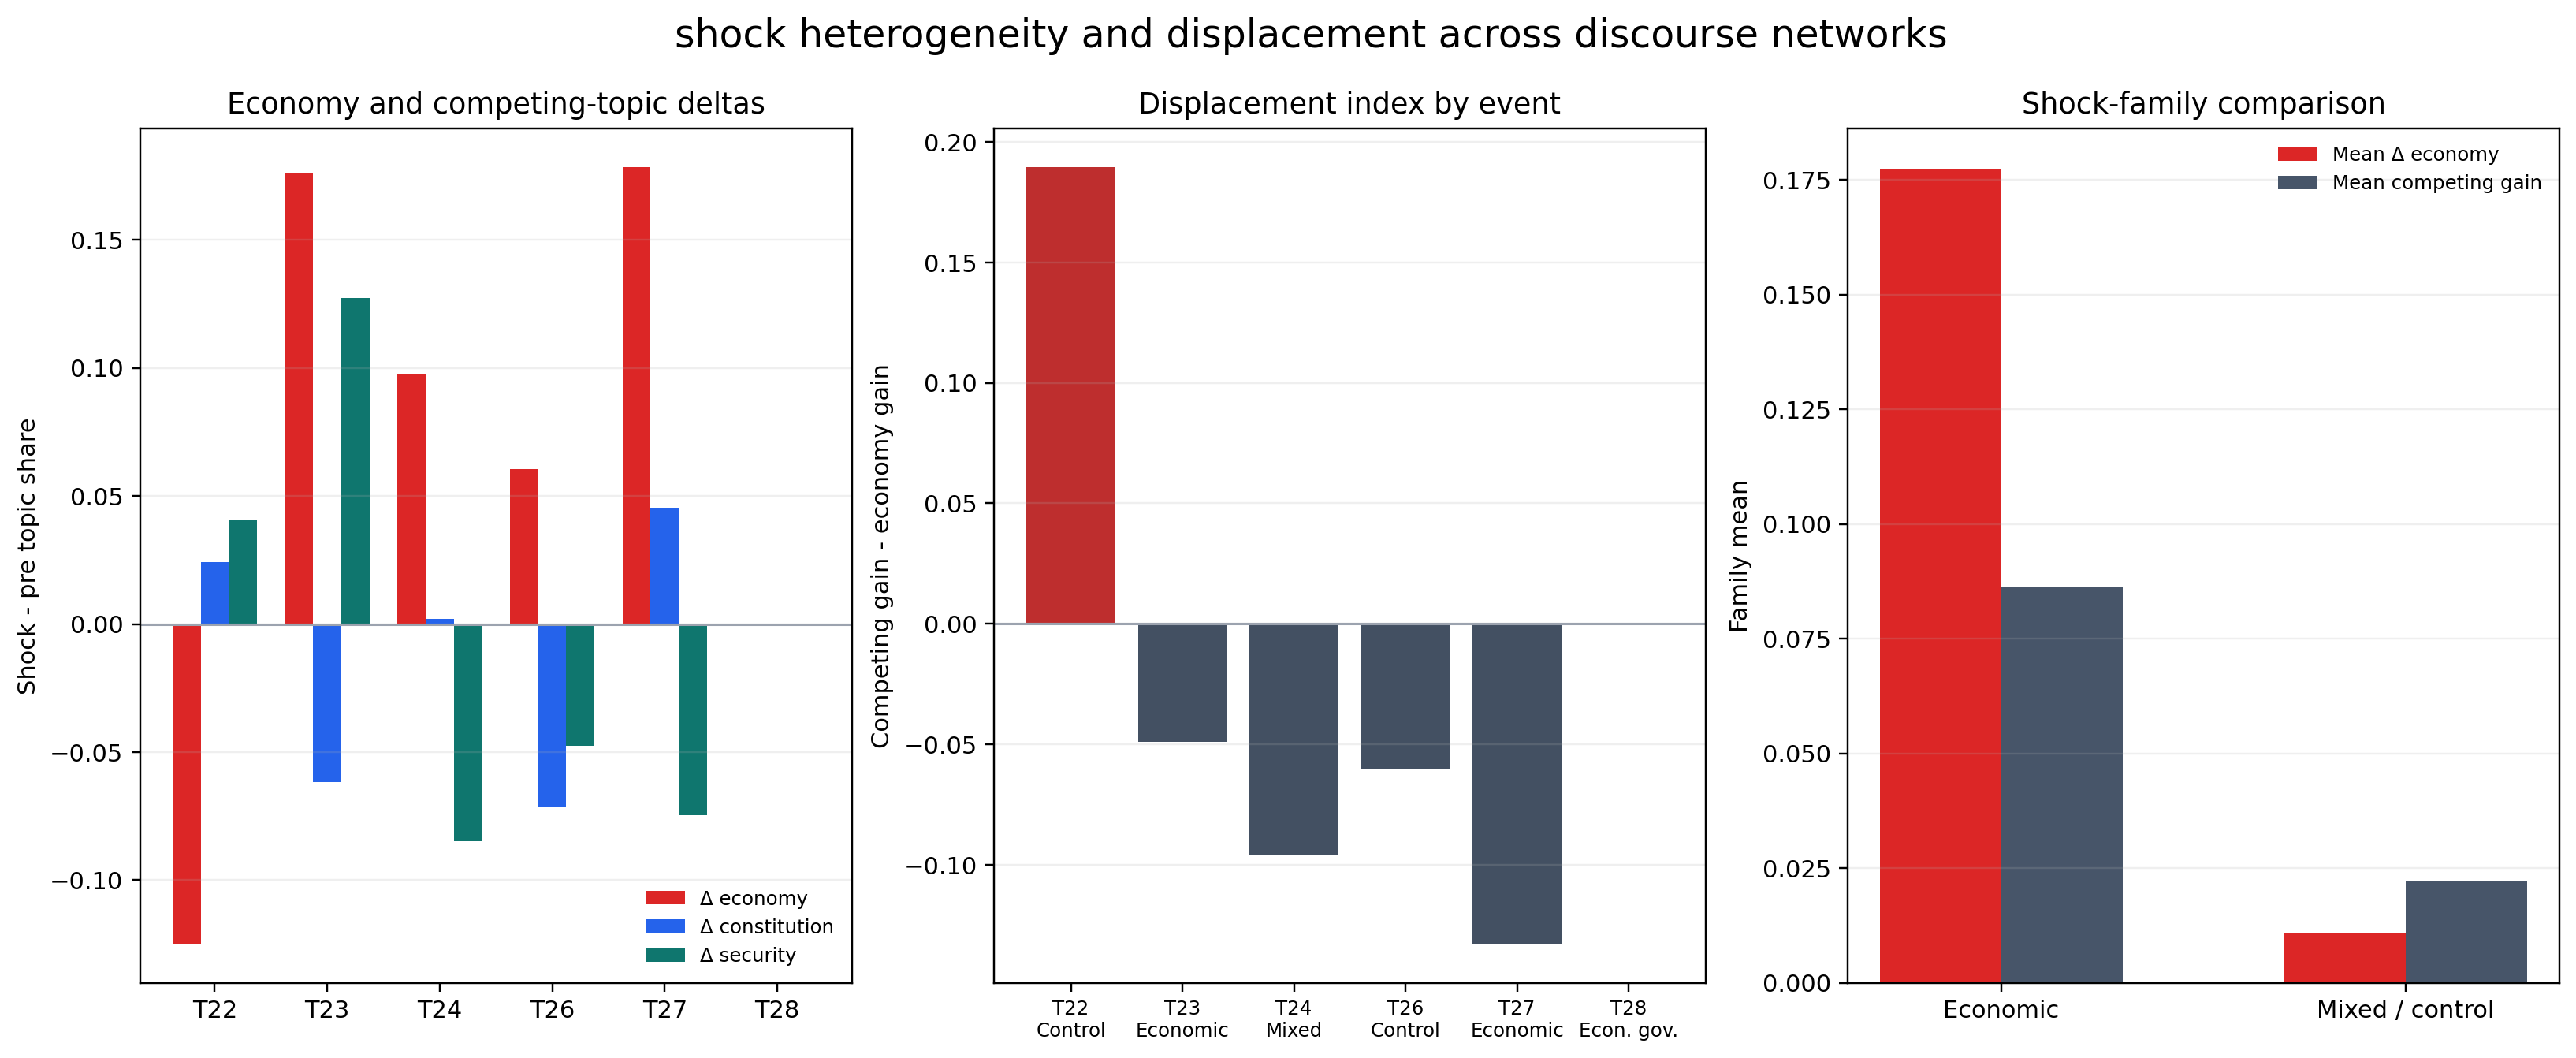
\includegraphics[width=\linewidth]{figure_8_inter_term_shock_comparison.png}
    \caption{Shock heterogeneity and displacement. Events are labeled by shock family: Economic, Econ.\ gov.\ (economic-governance), Mixed, or Control. Center panel: the displacement index $DI_e$ by event, competing-topic gains minus the economy's own gain; positive means competing topics gained more during the shock (the economy was partly crowded out), negative means the economy's own gain was larger. Core economic shocks maintain negative displacement; mixed events flip it positive.}
    \label{fig:heterogeneity}
\end{figure}

\subsection{The Common Economic Axis Makes Inter-Term Comparison Defensible}
The pooled latent axis is strongly interpretable. The economy feature has the largest positive weight, followed by interest and inflation, while IMF/external finance loads in the opposite direction. The axis correlates strongly with the anchor ordering ($r=0.711$) and stays stable under bootstrap and leave-one-anchor-out diagnostics.

This makes inter-term drift interpretable rather than decorative. AKP remains durably on the positive side of the axis and drifts further in that direction by Term 28. CHP moves from near-center or slightly positive placement in Term 22 to clearly negative positions in Terms 27 and 28. The value of the common axis is not that it reduces politics to one dimension, but that it puts otherwise separate term-level geometries onto a shared scale.

\begin{figure}[htbp]
    \centering
    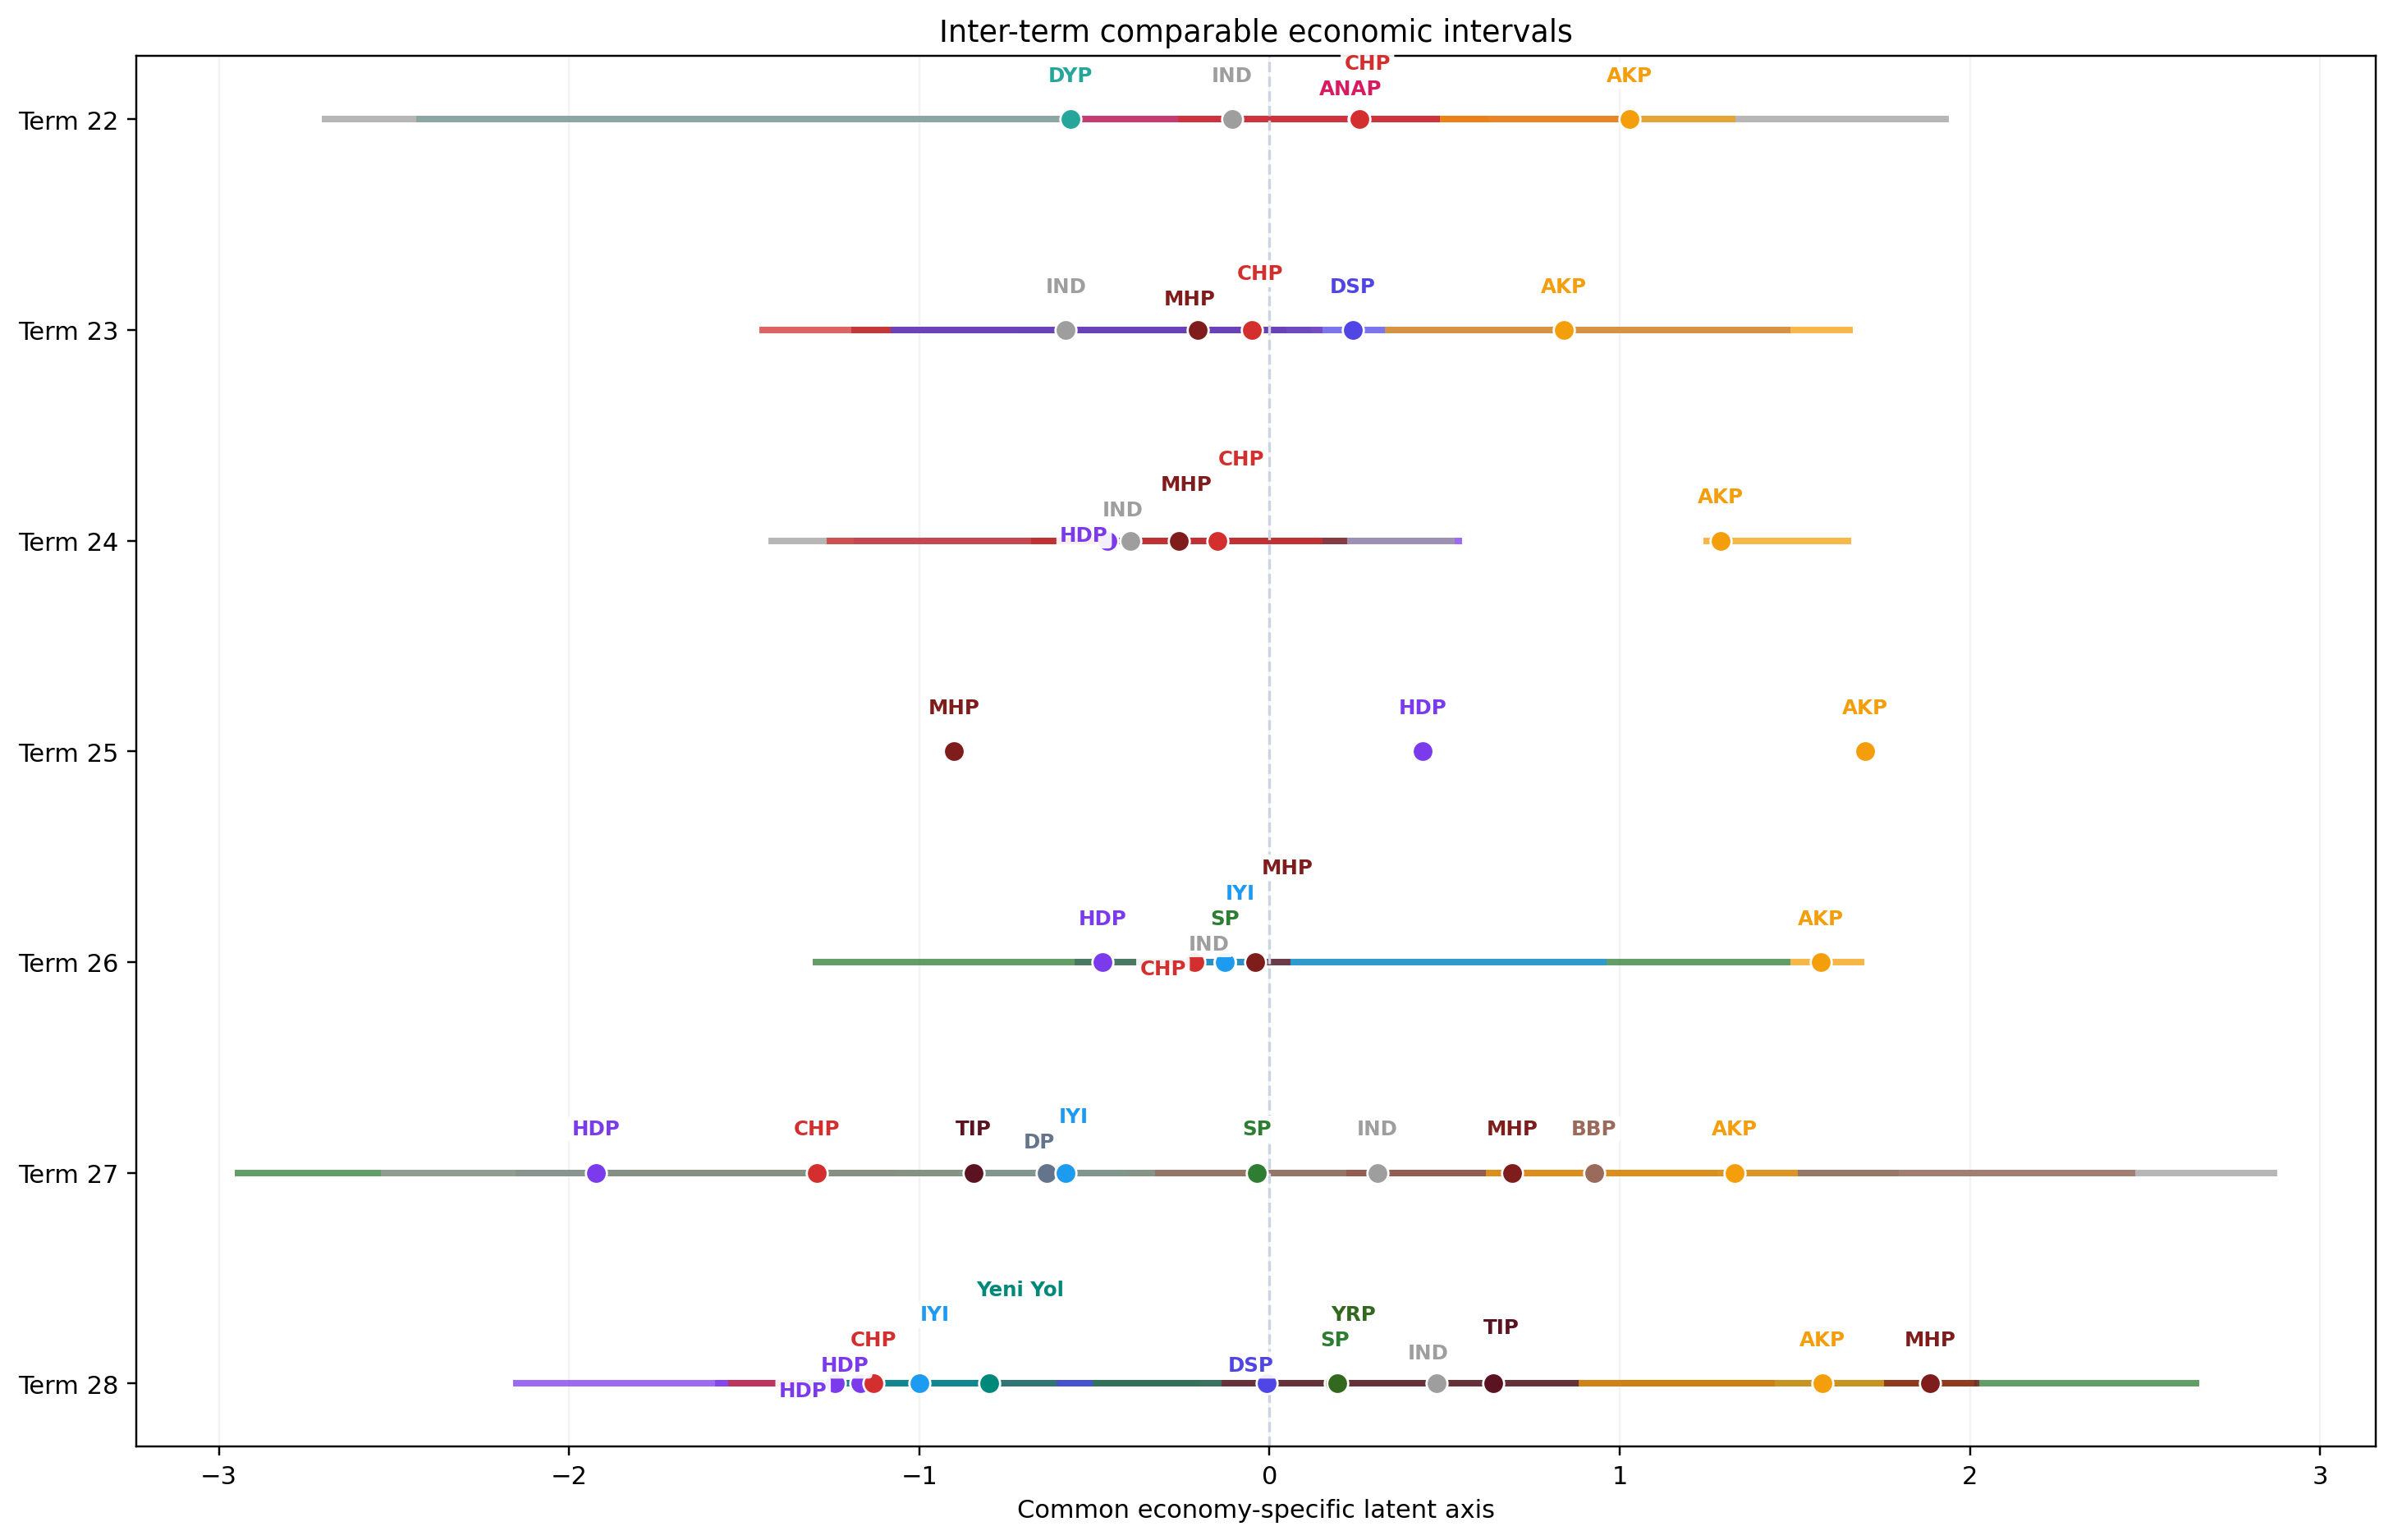
\includegraphics[width=\linewidth]{figure_2_inter_term_economic_latent_axis.png}
    \caption{Common inter-term economic latent axis. A party's position on this axis is a single summary score per party per term, combining how positively or negatively \emph{and} how often that party discusses economic topics, placed on one common scale so positions are comparable across terms. Each party-term interval shows the within-term range and central tendency of that party's economic discourse position on the pooled axis. Parties are consistent in color across terms.}
    \label{fig:interterm_axis}
\end{figure}

\section{Robustness Checks}
Because the analysis relies on discourse rather than roll-call behavior, robustness must be made explicit. The strongest salience shocks survive comparison with within-term placebo months. The Term 23 global crisis reaction and the Term 27 FX crisis produce economy-salience deviations with z-scores of 2.89 and 2.79 relative to their local null baselines, making them unusual even in crisis-saturated terms.

Axis stability is also strong. The observed anchor correlation is 0.711, the permutation p-value is effectively zero, the bootstrap mean anchor correlation is 0.674 with standard deviation 0.077, and the minimum leave-one-anchor-out correlation with the full axis remains 0.972. These checks do not prove the paper's interpretation automatically, but they show that the main results are not reducible to arbitrary anchor choice, one influential party, or ordinary month-to-month noise.

\begin{figure}[htbp]
    \centering
    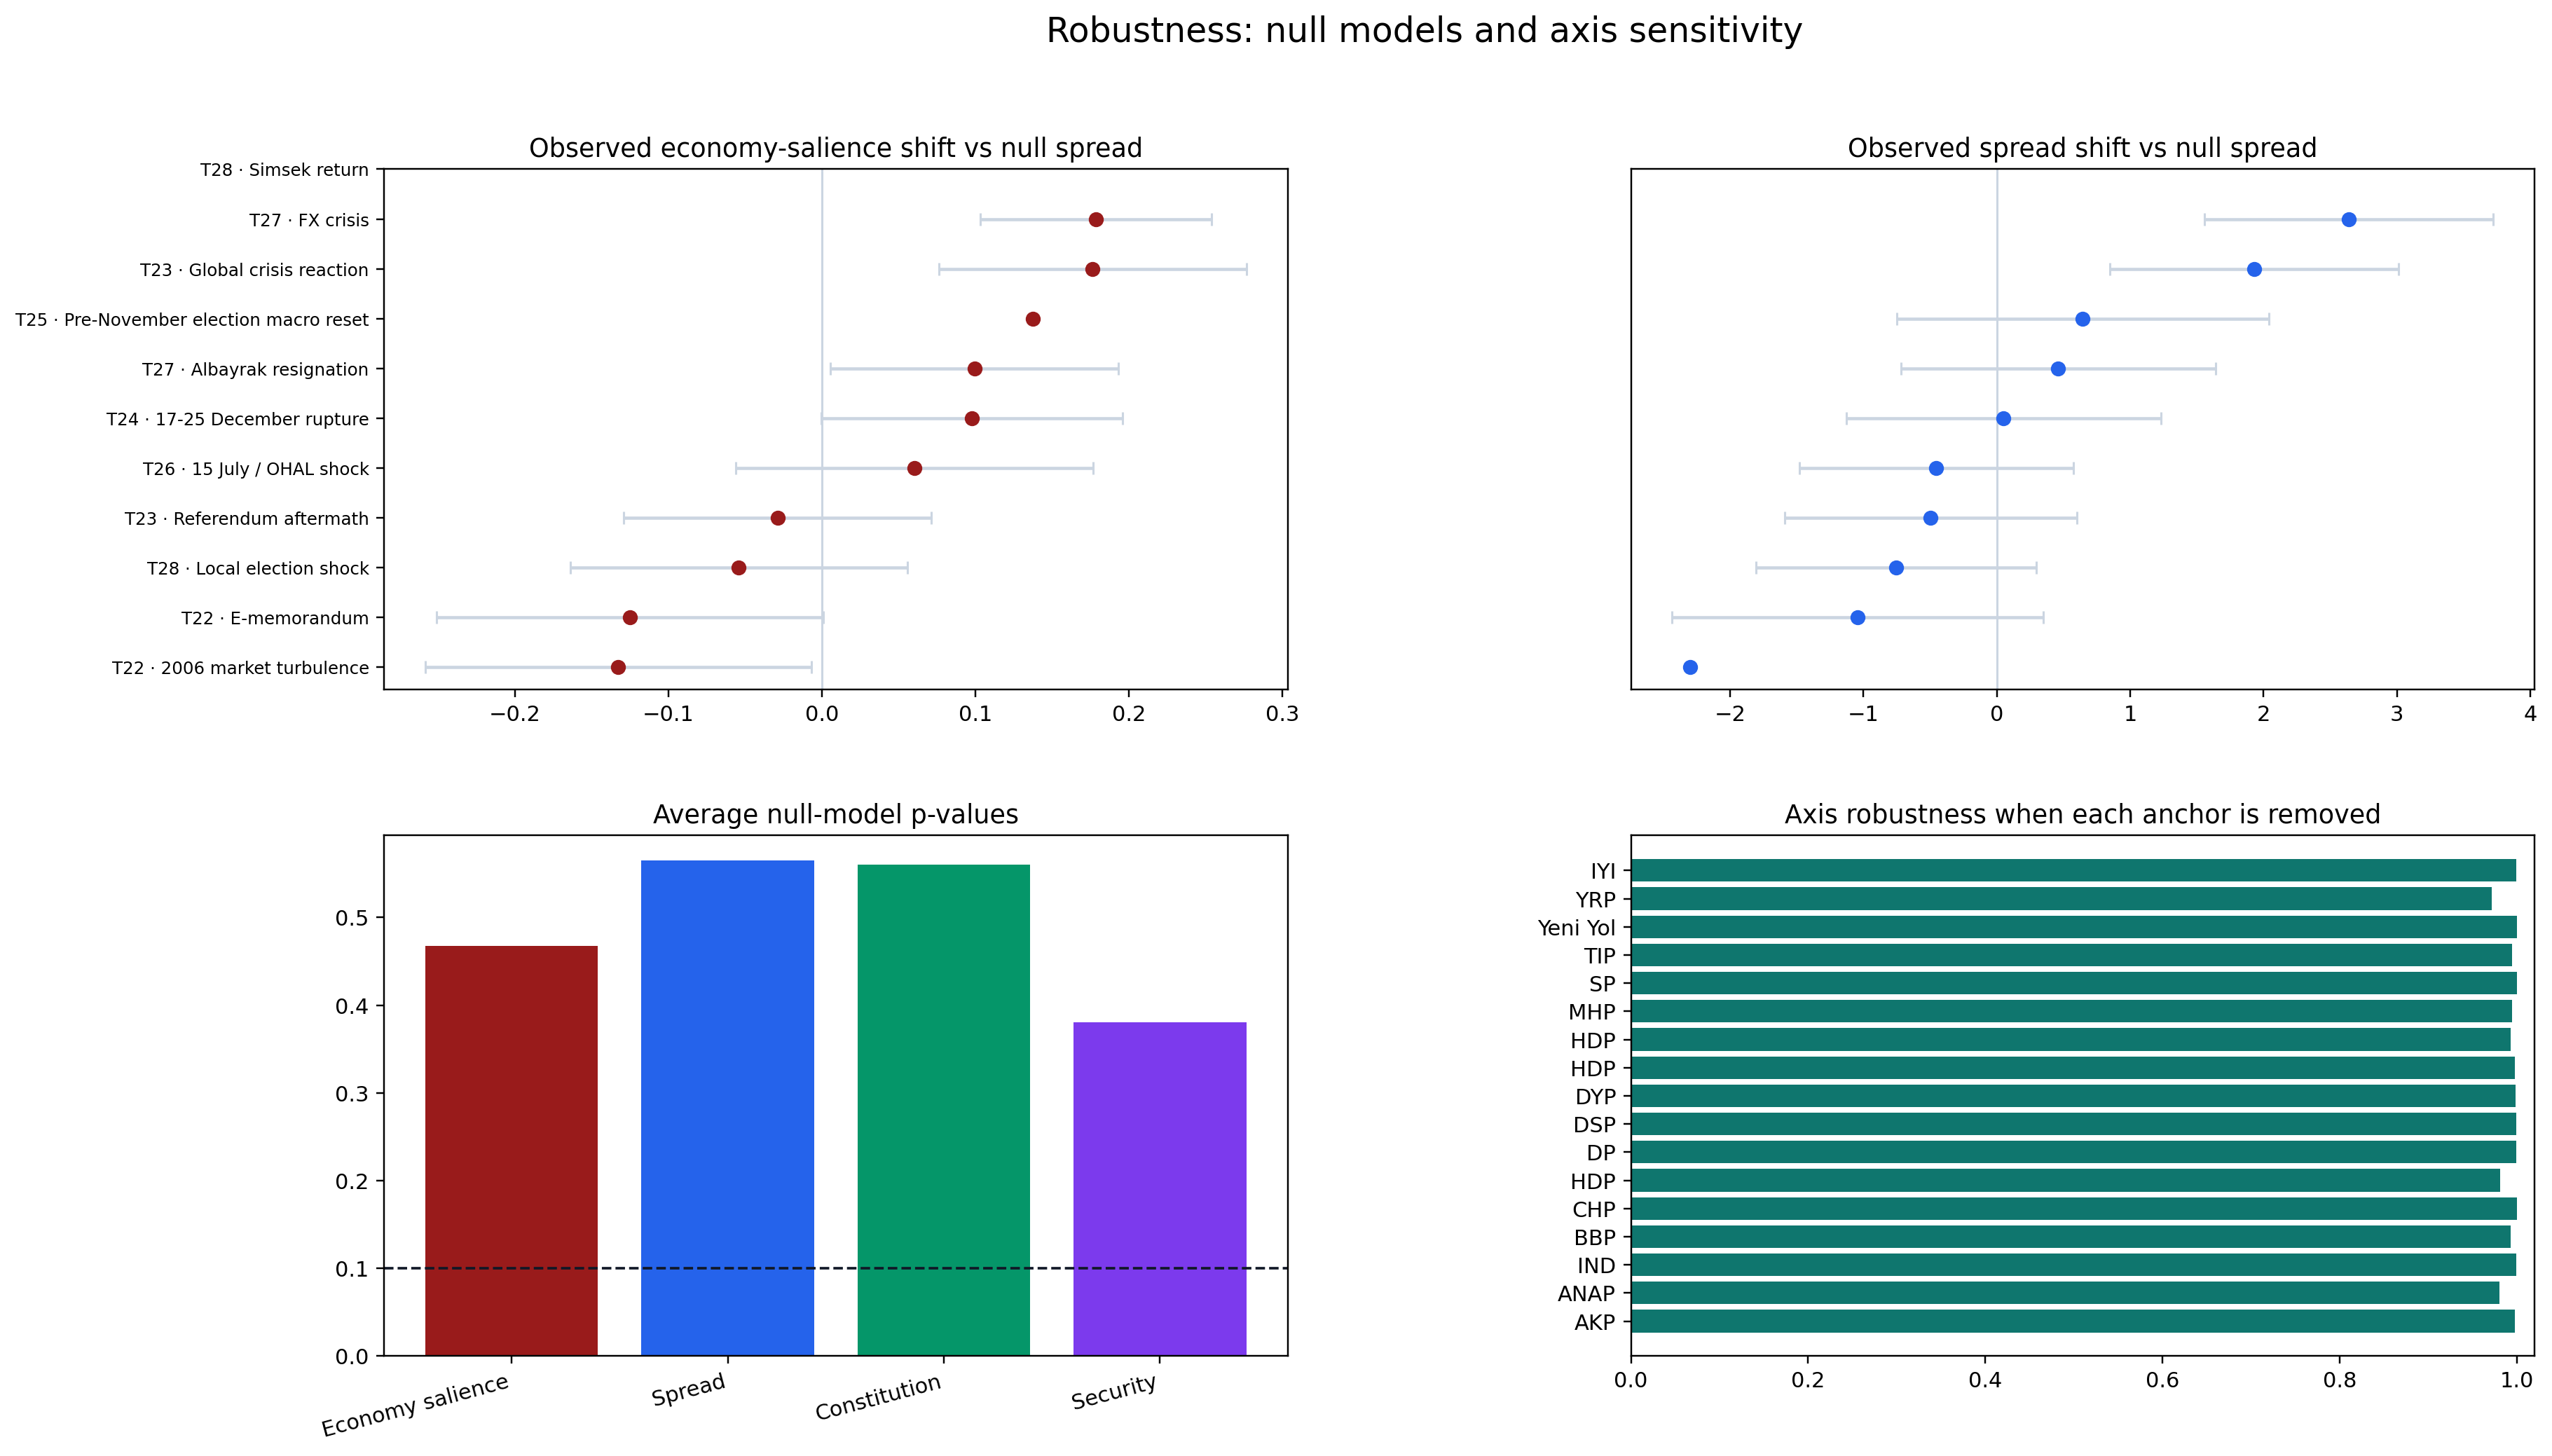
\includegraphics[width=\linewidth]{figure_9_robustness_null_models.png}
    \caption{Robustness and null-model panel. A \emph{placebo contrast} recomputes the same pre-versus-shock comparison for ordinary, non-shock months, giving a null range of month-to-month change against which each event's real shock-window change (top row) is checked. Bottom row: null-model p-values by quantity (left) and latent-axis stability when each anchor is removed (right). These diagnostics evaluate whether the main results exceed routine monthly fluctuation.}
    \label{fig:robustness}
\end{figure}

\section{Discussion}
Four broader conclusions follow from this analysis. First, economic shocks are not simple volume shocks. They alter who owns the discourse, how far apart parties are, and who can bridge the field. Second, ownership is not a fixed property of either the government or the opposition -- it can move to the government, stay with the opposition, or be reallocated within the opposition itself. Third, partisan reconfiguration is heterogeneous: some shocks widen the field, while others compress it into a more tightly shared crisis vocabulary. Fourth, constitutional and security crises can suppress economic centrality even when macroeconomic pressure is objectively present.

The design is deliberately portable. Its required inputs are parliamentary speech, timestamps, party labels, a topic family definition, and a monthly macroeconomic series. That makes it transferable to settings where speech data are easier to obtain than comprehensive roll-call infrastructure. The design does not solve every causal identification problem, but it provides a disciplined framework for comparing shock-driven discourse reorganization across legislatures.

This portability points toward concrete extensions. Parliaments with comparably open, full-text plenary archives -- the German Bundestag's plenary protocols, the UK House of Commons's Hansard, and the US Congressional Record -- are natural candidates for the same pipeline, applied to other party systems and shock histories. The same logic extends across policy domains, not only across legislatures: making security, migration, climate, or constitutional crises the primary object of study requires redefining only the topic and concept-keyword layer of Section~3. The underlying formalism -- the signed agenda feature, agenda ownership, party-party affinity and distance, structural brokerage, and the displacement index -- is domain-agnostic and carries over unchanged; the engine stays fixed, and only the topic vocabulary changes per language, parliament, or domain. The longer-term goal is to package this pipeline as a reusable, configurable tool for comparative parliamentary discourse analysis under shock conditions.

There are clear limits. The paper studies discourse networks, not legislative behavior networks. Topic families are theory-guided and validated within the project, but comparative reuse would require careful translation into the vocabulary of the destination parliament. The \c{S}im\c{s}ek return in Term 28 is substantively important but temporally asymmetric, so its ownership and brokerage evidence is stronger than its triptych comparability.

\section{Conclusion}
External economic shocks reorganize parliamentary discourse networks rather than simply making them louder. In the Turkish case, they raise or suppress economic salience, reallocate ownership of economic speech, widen or compress partisan geometry, and reassign the actors who bridge opposing blocs. Those dynamics are heterogeneous across event families and become visible once economic shocks are analyzed with explicit pre-shock, shock, and post-shock windows. More broadly, the paper demonstrates that discourse-only parliamentary network analysis can support portable causal claims when the signed feature layer, inter-term scale, and robustness tests are made explicit.

\begin{thebibliography}{00}
\bibitem{newman2018}
M. E. J. Newman, \emph{Networks}. Oxford University Press, 2018.

\bibitem{barabasi2016}
A.-L. Barabasi, \emph{Network Science}. Cambridge University Press, 2016.

\bibitem{menczer2020}
F. Menczer, S. Fortunato, and C. A. Davis, \emph{A First Course in Network Science}. Cambridge University Press, 2020.

\bibitem{bonchi2019}
F. Bonchi, E. Galimberti, A. Gionis, B. Ordozgoiti, and G. Ruffo, ``Discovering polarized communities in signed networks,'' 2019.

\bibitem{garimella2018}
K. Garimella, G. De Francisci Morales, A. Gionis, and M. Mathioudakis, ``Political discourse on social media: Echo chambers, gatekeepers, and the price of bipartisanship,'' 2018.

\bibitem{gionis2024}
A. Gionis, L. Oettershagen, and I. Sarpe, ``Mining temporal networks,'' 2024.

\bibitem{blohm2026}
P. Blohm, F. Chen, A. Gionis, and S. Neumann, ``Discovering opinion intervals from conflicts in signed graphs,'' 2026.

\bibitem{laver2003}
M. Laver, K. Benoit, and J. Garry, ``Extracting policy positions from political texts using words as data,'' \emph{American Political Science Review}, vol. 97, no. 2, pp. 311--331, 2003.

\bibitem{kleinnijenhuis1995}
J. Kleinnijenhuis and E. Rietberg, ``Parties, media, the public and the economy,'' \emph{European Journal of Political Research}, vol. 28, no. 1, pp. 95--118, 1995.

\bibitem{porter2005}
M. A. Porter, P. J. Mucha, M. E. J. Newman, and C. M. Warmbrand, ``A network analysis of committees in the United States House of Representatives,'' \emph{Proceedings of the National Academy of Sciences}, vol. 102, no. 20, pp. 7057--7062, 2005.
\end{thebibliography}

\end{document}
